\documentclass{article}

\usepackage[utf8]{inputenc}
\usepackage{enumitem}
\usepackage{multirow}
\usepackage{xcolor}
\usepackage[T1]{fontenc}
% \usepackage[french]{babel}
\usepackage{hyperref}
\usepackage{amssymb}
\usepackage{mathtools}
\usepackage{ntheorem}
\usepackage{amsmath}
\usepackage{amssymb}
\usepackage[ a4paper, hmargin={2cm, 2cm}, vmargin={3cm, 3cm}]{geometry}
\usepackage{capt-of}
\usepackage{multicol}
\usepackage{mathpartir}

\usepackage[braket, qm]{qcircuit}
\usepackage{graphicx}

\usepackage{tikz}
\usetikzlibrary{angles,quotes, 3d}

\usepackage{hyperref}
\hypersetup{
    colorlinks,
    citecolor=black,
    filecolor=black,
    linkcolor=blue,
    urlcolor=blue
}

\usepackage{xcolor}

\definecolor{codegreen}{rgb}{0,0.6,0}
\definecolor{codegray}{rgb}{0.5,0.5,0.5}
\definecolor{codepurple}{rgb}{0.58,0,0.82}

\usepackage{listings}
\lstdefinestyle{mystyle}{
    commentstyle=\color{codegreen},
    keywordstyle=\color{magenta},
    numberstyle=\tiny\color{codegray},
    stringstyle=\color{codepurple},
    basicstyle=\ttfamily\footnotesize,
    breakatwhitespace=false,
    breaklines=true,
    captionpos=b,
    keepspaces=true,
    numbers=left,
    numbersep=5pt,
    showspaces=false,
    showstringspaces=false,
    showtabs=false,
    tabsize=2
}
\lstset{style=mystyle}

\theoremstyle{plain}
\theorembodyfont{\normalfont}
\theoremseparator{~--}
\newtheorem*{proof}{Proof}
\newtheorem*{exam}{Example}
\renewcommand\qedsymbol{$\square$}

\newtheorem*{defi}{Definition}
\newtheorem{exo}{Exercise}[section]
\newtheorem{ans}{Answer}[section]
\newtheorem{lemma}{Lemma}[section]

\newcommand{\toto}{\twoheadrightarrow}

\newcommand{\rbeta}{\to_\beta}
\newcommand{\rsbeta}{\to_\beta^*}

\newcommand{\Mlambda}{{\underline \Lambda}}
\newcommand{\mlambda}{{\underline \lambda}}
\newcommand{\mbeta}{{\underline \beta}}
\newcommand{\tombeta}{\to_\mbeta}
\newcommand{\tosmbeta}{\to_\mbeta^*}


\title{$\lambda$-calculus}
\author{Thibaut BALABONSKI\\ \scriptsize noted by Valeran MAYTIE}
\date{}

\begin{document}
  \maketitle

  \tableofcontents

  \newpage
  \begin{itemize}
    \item 1935 (a theory of computable functions)

      Alonzo Church, attempt at formalizing computation
  \end{itemize}

  Functions:
  \begin{itemize}
    \item maths : $f : A \to B$ is a set of pairs
    \item programming : instruction to compute an output
  \end{itemize}

  \subsection{Definitions}

  We can define the set of $\lambda$-terms ($\Lambda$) with a grammar:
  \begin{align*}
    \Lambda :=&\; x, y, z ...         & (\text{variable}) \\
             |&\; \lambda. \Lambda    & (\text{functions}) \\
             |&\; \Lambda\; \Lambda   & (\text{application})
  \end{align*}

  The application is left associative: $(l_1\; l_2)\; l_3$.

  \paragraph{Notations} We can define some notations to simplify the syntax :

  \begin{center}
  \begin{tabular}{ c|c }
    Real $\lambda$-term & notations \\
    \hline
    $\lambda x_1.(\ldots(\lambda x_n. t)\ldots)$ & $\lambda x_1 \ldots
    \lambda x_n. t$ \\
    $(\ldots (t\; u_1)\ldots)$ & $t\;u_1 \ldots u_n$ \\
    $t\; u_1\; \ldots_; u_n$ & $t\; \vec{u}$ with $\vec u = u_1\; \ldots\; u_n$
  \end{tabular}
  \end{center}

  \exam We can define this $\lambda$-term:

  \begin{itemize}
    \item Identity : $I = \lambda x.\; x$
    \item Constant generator: $C_c = \lambda x.\; c$
    \item Distribution : $\lambda x\; y\; z.\; (x\;z)\; (y\;z)$
    \item What ? : $\delta = \lambda x.\;x\;x$
  \end{itemize}


  \paragraph{Curryfication} Functions are curryfied (Haskell Curry)

  They are no cartesian product in the $\lambda$-calculus. So we can define :

  \begin{center}
  \begin{tabular}{l l l}
    $\bullet$ A function: & $(x, y)\mapsto t$ & $\lambda x\;y.\; t$ \\
    $\bullet$ An application & $f(x, y)$ & $f\; x\; y$
  \end{tabular}
  \end{center}

  \section{Computing with the $\lambda$-calculus}

  Example, we want to compute $(\lambda x y z.\; x\; z\; (y\; z))\; (\lambda a
  b.\; a)\; t\; u$

  \begin{align*}
    &\;(\lambda x y z.\; x\; z\; (y\; z))\; (\lambda a b.\; a)\; t\; u \\
    =&\;(\lambda y z.\; (\lambda a b.\; a)\; z\; (y\; z))\; t\; u \\
    =&\;(\lambda z.\; (\lambda a b.\; a)\; z\; (t\; z))\; u \\
    =&\;(\lambda a b.\; a)\; u\; (t\; u))\\
    =&\;(\lambda b.\; u)\; (t\; u))\\
    =&\;u
  \end{align*}

  Here are some examples of slightly more subtle calculations:
  \begin{multicols}{2}
    \begin{align*}
      &(\lambda x.\; (\lambda x.\; x))\; y \\
      &=\; \lambda x.\; x
    \end{align*}

    \begin{align*}
      &(\lambda x.\; (\lambda y.\; x))\; y \\
      &=\; \lambda z.\; y
    \end{align*}
  \end{multicols}

  We will define the reduction rewrite rule called $\beta$-reduction later.

  \subsection{Inductive reasoning}

  We can also define $\Lambda$ with the smallest set such that :

  \begin{itemize}
    \item $\forall x \in \text{Var}, x \in \Lambda$
    \item $\forall x \in \text{Var}, \forall t \in \Lambda, \lambda x.t \in
      \Lambda$
    \item $\forall t_1 t_2, t_1\; t_2 \in \Lambda$
  \end{itemize}

  We define $\Lambda$ by induction, so we can write induction function.

  For example, we can write $f_v$ the function who compute the number of
  variable in term $t$ and $f_@$ the function who compute the number of
  application
  \begin{multicols}{2}
    \[
        \begin{cases}
            f_v(x) &= 1 \\
            f_v(\lambda x. t) &= f_v(t) \\
            f_v(t_1\; t_2) &= f_v(t_1) + f_v(t_2) \\
        \end{cases}
    \]

    \[
        \begin{cases}
            f_@(x) &= 0 \\
            f_@(\lambda x. t) &= f_@(t) \\
            f_@(t_1\; t_2) &= 1 + f_@(t_1) + f_@(t_2) \\
        \end{cases}
    \]
  \end{multicols}

  How to prove that some property $P(t)$ is valid for all $\lambda$-terms $t$ ?

  \begin{enumerate}
    \item Prove that $\forall x \in \text{Var}, P(x)$ is valid
    \item Prove that $\forall x \in \text{Var}, \forall t, P(t) \Rightarrow
      P(\lambda x.\; t)$ is valid
    \item Prove that $\forall t_1, t_2, P(t_1) \wedge P(t_2) \Rightarrow P(t_1
      \; t_2)$ is valid
  \end{enumerate}

  \exam We want to prove $H : \forall t, f_v(t) = 1 + f_@(t) $

  \proof We proof $H$ by induction on the term $t$ :

  \begin{itemize}
    \item $t = x$, $f_v(x) = x$ and $f_@(x) = 0$, so we have $f_v(x) = 1 +
      f_@(x)$

    \item $t = \lambda x. t$, we assume that $f_v(t) = 1 + f_@(t)$.
      We calculate $f_v(\lambda x. t) = f_v(t) = 1 + f_@(t) = 1 + f_@(\lambda
      x.t)$

    \item $t = t_1\; t_2$, we assume that $f_v(t_1) = 1 + f_@(t_1)$ and
      $f_v(t_2) = 1 + f_@(t_2)$. By the calculation $f_v(t_1\; t_2) = f_v(t_1) +
      f_v(t_2) = 1 + f_@(t_1) + 1 + f_@(t_2) = 1 + f_@(t_1\; t_2)$
  \end{itemize}
  \qedsymbol

  \subsection{Variables and substitutions}

  \subsubsection{Free and bound variables}

  To define more calculation operations, we define free variables and bound
  variables.

  Informally, free variables are variables used, but linked to no lambda
  abstraction. While linked variables are those used and linked to a lambda
  abstraction.

  Definition :

  \begin{multicols}{2}
    \[
      \begin{cases}
        fv(x) &= \{x\} \\
        fv(\lambda x. t) &= fv(t)\backslash \{x\} \\
        fv(u\; v) &= fv(u) \cup fv(v) \\
      \end{cases}
    \]

    \[
      \begin{cases}
        bv(x) &= \emptyset \\
        bv(\lambda x. t) &= \{x\} \cup bv(t) \\
        bv(u\; v) &= bv(u) \cup bv(v) \\
      \end{cases}
    \]
  \end{multicols}

  \subsubsection{Substitution}

  The substitution is an operation on $\lambda$-term. The aim is to replace the
  free occurrences of a variable $x$ in term $t$ with another $\lambda$-term
  $u$. It is noted : $t\{x \leftarrow u\}$. We can define this operation by
  induction on a $\lambda$-term :

  \begin{align*}
    y\{x \leftarrow y\} &= \begin{cases}
      u & \text{if } x = y \\
      y & \text{if } x \not = y
    \end{cases} \\
    (t_1\; t_2)\{y \leftarrow u\} &= t_1\{y \leftarrow u\}\; t_2\{y \leftarrow
    u\} \\
    (\lambda y.\;t)\{x \leftarrow u\} &= \begin{cases}
      \lambda y.\;t &\text{if } x = y \\
      \lambda y.\;t\{x\leftarrow u\} &\text{if } x \not = y \text{ and } y \not
      \in fv(u)\\
      \lambda z.\;t\{y\leftarrow z\}\{x\leftarrow u\} &\text{if } x \not = y \text{ and } y \in
      fv(u) \text{\hspace{1cm}$z$ fresh}\\
    \end{cases}
  \end{align*}

  \paragraph{Barendregt's convention} The definition of substitution above is
  not very easy to handle. So we are going to use a convention to greatly
  simplify the substitution :

  \begin{center}
    \textit{no variable name appears both free and bound in any given subterm}
  \end{center}

  \begin{center}
    \begin{tabular}{c|c}
      Good & Not Good \\
      \hline
      $\lambda x.\;x\;(\lambda x.\;x)$ & $\lambda x.\;(x\;(\lambda y.\;y))$
    \end{tabular}
  \end{center}

  The substitution definition become :

  \begin{align*}
    y\{x \leftarrow u\} &= \begin{cases}
      u & \text{if } x = y \\
      y & \text{if } x \not = y
    \end{cases} \\
    (t_1\; t_2)\{y \leftarrow u\} &= t_1\{y \leftarrow u\}\; t_2\{y \leftarrow
    u\} \\
    (\lambda y.\;t)\{x \leftarrow u\} &= \lambda y.\; t\{x \leftarrow u\}
  \end{align*}

  \paragraph{(Un)stability of Barendregt's convention}
  Sometimes during the computation we need to change variables name to preserve
  the convention :

  \begin{align*}
    &(\lambda x.\;x\;x)\;(\lambda yz.\;y\;z)\\
    &\to (\lambda yz.\;y\;z)\;(\lambda yz.\;y\;z)\\
    &\to (\lambda yz.\;(\lambda yz.\;y\;z)\;z) & \text{Wrong}\\
  \end{align*}

  \subsubsection{$\alpha$-conversion}

  Two term can be structurally different, but with the same meaning ($\lambda
  x.\; x$ and $\lambda y.\; y$). We can therefore rename linked variables under
  certain conditions without changing the meaning of a lambda term. We call this
  operation $\alpha$-conversion or $\alpha$-renaming.

  $\alpha$-conversion definition :

  \begin{align*}
    \lambda x.\; t &=_\alpha \lambda y.\;{x \leftarrow y} & \text{with } x,y
      \not \in bd(t) \text{ and } y \not \in fv(t)
  \end{align*}

  The $\alpha$-conversion is a congruence :

  \begin{align*}
    t =_\alpha t' &\Rightarrow \lambda x.\;t =_\alpha t' \\
    t_1 =_\alpha t_1' &\Rightarrow t_1\;t_2 =_\alpha t_1'\;t_2 \\
    t_2 =_\alpha t_2' &\Rightarrow t_1\;t_2 =_\alpha t_1\;t_2' \\
  \end{align*}

  From now on we assume that any term we work with satisfies Barendregt’s
  convention.

  \exo Make them nice
    \begin{itemize}
      \item $\lambda x.\; (\lambda x.\; x\; y) (\lambda y. x\; y)$
      \item $\lambda x y.\; x (\lambda y.\; (\lambda y.\; y)\; y\; z)$
    \end{itemize}

  \textit{Answer :}
    \begin{itemize}
      \item $\lambda x.\; (\lambda x.\; x\; y) (\lambda y. x\; y) =_\alpha
        \lambda x.\; (\lambda z.\; z\; y) (\lambda w. x\; w)$
      \item $\lambda x y.\; x (\lambda y.\; (\lambda y.\; y)\; y\; z) =_\alpha
        \lambda x y.\; x (\lambda a.\; (\lambda t.\; t)\; a\; z)$
    \end{itemize}

  \exo Compute $(\lambda f.\; f\;f)\; (\lambda a b. b\;a\;b)$

  \textit{Answer :}
    \begin{align*}
      (\lambda f.\;f\;f)\; (\lambda a\; b.\;b\;a\;b) &\to_\beta
      (\lambda a b.\;b\;a\;b)\; (\lambda a\;b.\;b\;a\;b) \\
      &\to_\beta \lambda b.\;b\;(\lambda a\;b.\;b\;a\;b)\;b\\
      &=_\alpha \lambda b.\;b\;(\lambda x\;y.\;y\;x\;y)\;b\\
      &\to_\beta \lambda b.\;b\;(\lambda y.\;y\;b\;y)\\
    \end{align*}


  \exo Prove that $fv(t[x \leftarrow u]) \subseteq (fv(t) \backslash \{x\})
    \cup fv(u)$

  \textit{Answer :} Proof by induction on the structure of $t$

  \begin{itemize}
    \item Case where $t$ is a variable
      \begin{itemize}
        \item case x: $fv(x\{x\leftarrow u\}) = fv(u) \subseteq (fv(t)
          \backslash \{x\} \cup fv(u)$
        \item case $y\not =x$: $fv(y\{x\leftarrow u\} ) fv(y) = \{y\}$ and
          $\{y\}$ is indeed a subset of ($fv(y)\backslash \{x\}) \cup fv(u) =
          \{y\} \cup fv(u)$)
      \end{itemize}

    \item case where $t$ is an application $t_1\;t_2$. Assume
      $fv(t_1\{x\leftarrow y\})\subseteq fv(t_1) \backslash \{x\} \cup fv(u)$ and
      $fv(t_2\{x\leftarrow y\})\subseteq fv(t_2) \backslash \{x\} \cup fv(u)$.
      Then

      \begin{align*}
        &fv((t_1\;t_2)\{x \leftarrow u\}) \\
        &= fv(t_1\{x \leftarrow u\}\; t_2\{x \leftarrow u\}) & \text{by
        definition of the substitution} \\
        &= fv(t_1\{x \leftarrow u\}) \cup fv(t_2)\{x \leftarrow u\}) & \text{by
        definition of $fv$} \\
        &\subseteq fv(t_1 \backslash \{x\} \cup fv(u) \cup
        fv(t_2 \backslash \{x\} \cup fv(u) & \text{by induction hypothesis} \\
        &=fv(t_1 \backslash \{x\} \cup fv(t_2) \backslash \{x\}
        \cup fv(u) \\
        &=(fv(t_1 \cup fv(t_2)) \backslash \{x\}
        \cup fv(u) \\
        &= (fv(t_1\;t_2) \backslash \{x\}) \cup fv(u)
      \end{align*}

    \item Case where $t$ is $\lambda$-abstraction $\lambda y.t_0$. Asume
      $fv(t_0\{x\leftarrow u\} \subseteq (fv(t_0) \backslash \{x\} \cup fv(u)$.
      Then

      \begin{align*}
        &fv(\lambda y.t_0)\{x \leftarrow u\} \\
        &= fv(\lambda y.t_0\{x \leftarrow u\}) \\
        &= fv(t_0\{x \leftarrow u\})\{y\} \\
        &\subseteq ((fv(t_0) \backslash\{x\})\cup fv(u))\backslash \{y\} &
        \text{induction hypothesis} \\
        &= (fv(t_0) \backslash\{x\} \backslash \{y\})\cup fv(u)\backslash \{y\}
        \\
        &= (fv(t_0) \backslash\{x\} \backslash \{y\})\cup fv(u) \\
        &= (fv(t_0) \backslash \{y\} \backslash\{x\})\cup fv(u) \\
        &= (fv(\lambda y.t_0) \backslash \{x\} \cup fv(u) \\
      \end{align*}
  \end{itemize}
  \qedsymbol

  \exo \label{exo:commsubst} Prove when $x\not\in fv(v)$ and $x \not = y$ then
  $t\{x\leftarrow u\}\{y\leftarrow v\} = t\{y\leftarrow v\}\{x\leftarrow u\{y\leftarrow v\}\}$

  \textit{Answer} Proof by induction on $t$
  \begin{itemize}
    \item Case where $t$ is a variable $z$:
      \begin{itemize}
        \item $z = x$ :
          \begin{multicols}{2}
            \begin{align*}
              &x\{x\leftarrow u\}\{y\leftarrow v\} \\
              &= u\{y\leftarrow v\} \\
            \end{align*}

            \begin{align*}
              &x\{y\leftarrow v\}\{x\leftarrow u\{y\leftarrow v\}\} \\
              &= x\{x\leftarrow u\}\{y\leftarrow v\}\} \\
              &= u\{y\leftarrow v\} \\
            \end{align*}
          \end{multicols}

        \item $z = y$ :
          \begin{multicols}{2}
            \begin{align*}
              &y\{x\leftarrow u\}\{y\leftarrow v\} \\
              &= y\{y\leftarrow v\} \\
              &= v \\
            \end{align*}

            \begin{align*}
              &y\{y\leftarrow v\}\{x\leftarrow u\{y\leftarrow v\}\} \\
              &= v\{x\leftarrow u\{y\leftarrow v\}\} \\
              &= v & \text{$x$ is not free in $v$} \\
            \end{align*}
          \end{multicols}
        \item $z \not = y$ and $z \not = x$ :
          $z\{x\leftarrow u\}\{y\leftarrow v\} = z$ and
          $z\{y\leftarrow v\}\{x\leftarrow u\{y\leftarrow v\}\} = z$
      \end{itemize}

    \item $t = t_1\; t_2$:
      \begin{align*}
        &(t_1\;t_2)\{x\leftarrow u\}\{y\leftarrow v\} \\
        &t_1\{x\leftarrow u\}\{y\leftarrow v\}\;t_2\{x\leftarrow u\}\{y\leftarrow v\} \\
        &t_1\{y\leftarrow v\}\{x\leftarrow u\{y\leftarrow v\}\}\;
         t_2\{y\leftarrow v\}\{x\leftarrow u\{y\leftarrow v\}\} &
         \text{induction hypothesis} \\
        &(t_1\;t_2)\{y\leftarrow v\}\{x\leftarrow u\{y\leftarrow v\}\}\\
      \end{align*}

    \item $t = \lambda z.\;t_0$
      \begin{align*}
        &(\lambda z.\;t_0)\{x\leftarrow u\}\{y\leftarrow v\} \\
        &\lambda z.\;t_0\{x\leftarrow u\}\{y\leftarrow v\} \\
        &\lambda z.\;t_0\{y\leftarrow v\}\{x\leftarrow u\{y\leftarrow v\}\} &
        \text{induction hypothesis}\\
        &(\lambda z.\;t_0)\{y\leftarrow v\}\{x\leftarrow u\{y\leftarrow v\}\} \\
      \end{align*}

  \end{itemize}
  \qedsymbol

  \subsection{$\beta$-reduction}

    The $\beta$-reduction is a rewrite rule who apply an argument to a function.
    We need to have a $\lambda$-term on the form $(\lambda x.\;t)\; u$. This
    form is called a ($\beta$-redex). The computation rule is :
    \[(\lambda x.\;t)\; u \to_\beta t\{x \leftarrow u\}\]

    We can draw :

    \begin{center}
    \begin{tikzpicture}[line width=0.3mm]
      \node(App1) at (0, 0) {$@$};
        \node(Abs1) at (-2, -1) {$\lambda x$};
        \node(Abs10) at (-2, -2) {$\lambda y$};
        \node(App100) at (-2, -3) {$@$};
          \node(App1001) at (-3, -4) {$@$};
            \node(Var10011) at (-3.5, -5) {$x$};
            \node(Var10012) at (-2.5, -5) {$y$};
          \node(App1002) at (-1, -4) {$@$};
            \node(Var10021) at (-1.5, -5) {$x$};
            \node(Abs10022) at (-0.5, -5) {$\lambda z$};
            \node(Var100220) at (-0.5, -6) {$z$};

        \node(Abs2) at (2, -1) {$\lambda a$};
        \node(Abs20) at (2, -2) {$\lambda b$};
        \node(App200) at (2, -3) {$@$};
          \node(Var2001) at (1.5, -4) {$b$};
          \node(Var2002) at (2.5, -4) {$a$};

      \draw (App1) -- (Abs1) (App1) -- (Abs2)
            (Abs1) -- (Abs10) (Abs10) -- (App100) -- (App1001) -- (Var10011)
                                                     (App1001) -- (Var10012)
            (App100) -- (App1002) -- (Var10021)
                        (App1002) -- (Abs10022) -- (Var100220)
            (Abs2) -- (Abs20) -- (App200) -- (Var2001) (App200) -- (Var2002);
      \node at (4, -2.5) {$\rightarrow_\beta$};

      \node(Abs0) at (7, 0) {$\lambda y$};
      \node(App00) at (7, -1) {$@$};
        \node(App001) at (6, -2) {$@$};
          \node(Abs0011) at (5.5, -3) {$\lambda a$};
          \node(Abs00110) at (5.5, -4) {$\lambda b$};
          \node(App001100) at (5.5, -5) {$@$};
            \node(Var0011001) at (5, -6) {$b$};
            \node(Var0011002) at (6, -6) {$a$};

          \node(Var0012) at (6.5, -3) {$y$};
        \node(App002) at (8, -2) {$@$};
          \node(Abs0021) at (7.5, -3) {$\lambda a$};
          \node(Abs00210) at (7.5, -4) {$\lambda b$};
          \node(App002101) at (7.5, -5) {$@$};
            \node(Var0021011) at (7, -6) {$b$};
            \node(Var0021012) at (8, -6) {$a$};
          \node(Abs0022) at (8.5, -3) {$\lambda z$};
          \node(Var00220) at (8.5, -4) {$z$};

      \draw (Abs0) -- (App00) -- (App001) -- (Abs0011) -- (Abs00110) -- (App001100) -- (Var0011001)
                                                                        (App001100) -- (Var0011002)
                                 (App001) -- (Var0012)
                      (App00) -- (App002) -- (Abs0021) -- (Abs00210) -- (App002101) -- (Var0021011)
                                                                        (App002101) -- (Var0021012)
                                 (App002) -- (Abs0022) -- (Var00220);
    \end{tikzpicture}
    \end{center}

  A $\beta$-reduction can be done anywhere in a term. We must therefore manage
  cases where a reduction is made after a lambda abstraction or in the left or
  right branch of an application. So we're going to describe our reduction
  using inference rule :


  \begin{mathpar}
    \inferrule { }
      {(\lambda x.\;t)\; u \\ \to_\beta \\ t\{x \leftarrow u\}} \\
    \inferrule
      {t \\ \to_\beta \\ t'}
      {t\;u \\ \to_\beta \\ t'\; u} \and
    \inferrule
      {u \\ \to_\beta \\ u'}
      {t\;u \\ \to_\beta \\ t\; u'} \\
    \inferrule
      {t \\ \to_\beta \\ u'}
      {\lambda x.\;t \\ \to_\beta \\ \lambda x.\;t'}
  \end{mathpar}


  \subsubsection{Position}

  We can locate the beta reduction by encoding the position of the reduction
  operation, we can rewrite the resets like this :

  \begin{mathpar}
    \inferrule { }
      {(\lambda x.\;t)\; u \\ \xrightarrow{\epsilon}_\beta \\ t\{x \leftarrow u\}} \\
    \inferrule
      {t \\ \xrightarrow{p}_\beta \\ t'}
      {t\;u \\ \xrightarrow{1 \cdot p}_\beta \\ t'\; u} \and
    \inferrule
      {u \\ \xrightarrow{p}_\beta \\ u'}
      {t\;u \\ \xrightarrow{2 \cdot p}_\beta \\ t\; u'} \\
    \inferrule
      {t \\ \xrightarrow{p}_\beta \\ u'}
      {\lambda x.\;t \\ \xrightarrow{0 \cdot p}_\beta \\ \lambda x.\;t'}
  \end{mathpar}

  \subsubsection{Inductive reasoning on reduction}

    Since the $\beta$-reduction has been defined using inference rules, we can
    resonate by recurrence on the reduction. To prove a formula of the form :

    \[
      \forall t, t', t \to_\beta t' \Rightarrow P(t, t')
    \]

    we need to check the following four points:

    \begin{align*}
      &\bullet P((\lambda x.\;t)u, t\{x\rightarrow u\}) \text{ for any } x, y \text{ and
      } u \\
      &\bullet P(t\;u, t'\;u) \text{for any } t, t' \text{ and } u \text{ such that }
      P(t, t') \\
      &\bullet P(t\;u, t\;u') \text{for any } t, u \text{ and } u' \text{ such that }
      P(u, u') \\
      &\bullet P(\lambda x.\;t, \lambda x.\;t') \text{for any } x, t \text{ and } u' \text{ such that }
      P(t, t') \\
    \end{align*}

  \exam We want to prove :

    \[\forall t\;t', t \to t' \Rightarrow fv(t') \subseteq fv(t)\]

  Proof by induction on the derivation of $t \to t'$.

  \begin{itemize}
    \item $(\lambda x.\;t)\;u \to t\{x \leftarrow u\}$. We already proved:
      $fv(t\{x \leftarrow y\} \subseteq (fv(t) \backslash \{x\} \cup fv(u)$.
      Moreover, we have

      \begin{align*}
        fv((\lambda x.\;t)\;u) &= fv(\lambda x.\;t) \cup fv(u) \\
            &= (fv(t)\backslash \{x\}) \cup fv(u)
      \end{align*}
    \item $t\;u t'\; u$ with $t \to t'$. Then

      \begin{align*}
        fv(t'\;u) &= fv(t') \cup fv(u) & \text{by definition} \\
        &\subseteq fv(t) fv(u) & \text{by induction hypothesis} \\
        &= fv(t\; u) & \text{by definition}
      \end{align*}

    \item $t\; u' \to t\; u'$ with $u \to u'$ similar.

    \item $\lambda x.\;t \to \lambda x.\; t'$ with $t\to t'$. Then

      \begin{align*}
        fv(\lambda x.\; t') &= fv(t')\backslash\{x\} & \text{by definition} \\
        &\subseteq fv(t) \backslash \{x\} & \text{by induction hypothesis} \\
        &= fv(\lambda x.\; t) & \text{by definition}
      \end{align*}
  \end{itemize}
  \qedsymbol

  \subsubsection{Reduction sequences}

  Other reduction can be set above the beta reduction :

  \begin{itemize}
    \item $\to_\beta$ one step
    \item $\to_\beta^*$ reflexive transitive closure: 0, 1 or many steps
    \item $\leftrightarrow$ symmetric closure : one step, forward or backward.
    \item $=_\beta$ reflexive, symmetric, transitive closure (equivalence)
  \end{itemize}

  \subsubsection{Context}

  We can also formalize our reduction with a context that is intuitively a
  lambda term with a hole. So we have two steps, replace a variable with a hole
  and replace the hole with a lambda term. So there is no need for substitution.

  We define a context with the following grammar:

  \begin{align*}
    \mathcal C :=&\; \square              & (\text{hole})\\
             |&\; x, y, z ...             & (\text{variable}) \\
             |&\; \lambda x.\; \mathcal C & (\text{functions}) \\
             |&\; \mathcal C\; \mathcal C & (\text{application})
  \end{align*}

  The operation $\mathcal C[u]$ is the result of filling the hole of $\mathcal
  C$ with the term $u$.

  \exo Here are some decompositions of $\lambda x.(x\; \lambda y.xy)$ into a
  context and a term $\mathcal C[u]$

  \begin{center}
  \begin{tabular}{c|c|c|c|c|c}
    $\mathcal C$ & $\square$ & $\lambda x.\square$ & $\lambda x.(\square\;
    \lambda y.xy)$ & $\lambda x.(x\; \square)$ & $\ldots$ \\
    \hline
    $u$ & $\lambda x.(x\; \lambda y.xy)$ & $x\; \lambda y.xy$ & $x$ & $\lambda
    y.\; x\;y$ & $\ldots$
  \end{tabular}
  \end{center}

  What are the other possible decompositions ?

  We already showed that

  \[
    (\lambda x.x\; ((\lambda y.zy)x))z \to (\lambda x.x\; (zx))\; z
  \]
  What are the context and the redex associated to this reduction ?

  \textit{Answer} Other decompositions of $\lambda x.(x\; \lambda y.xy)$

  \begin{center}
  \begin{tabular}{c|c|c|c|}
    $\mathcal C$ & $\lambda x.(x\; \lambda y.\square)$ & $\lambda x.(x\; \lambda
    y.\square\; y)$ & $\lambda x.(x\; \lambda y. x\; \square)$ \\
    \hline
    $u$ & $xy$ & $x$ & $y$
  \end{tabular}
  \end{center}

  Decomposition of the reduction:

  \[
    \mathcal C[(\lambda y.xy)x] \to \mathcal C [zx]
  \]

  with $\mathcal C = (\lambda x.x\;\square)\;z$



  \section{Computing with the $\lambda$-calculus}

  Example, we want to compute $(\lambda x y z.\; x\; z\; (y\; z))\; (\lambda a
  b.\; a)\; t\; u$

  \begin{align*}
    &\;(\lambda x y z.\; x\; z\; (y\; z))\; (\lambda a b.\; a)\; t\; u \\
    =&\;(\lambda y z.\; (\lambda a b.\; a)\; z\; (y\; z))\; t\; u \\
    =&\;(\lambda z.\; (\lambda a b.\; a)\; z\; (t\; z))\; u \\
    =&\;(\lambda a b.\; a)\; u\; (t\; u))\\
    =&\;(\lambda b.\; u)\; (t\; u))\\
    =&\;u
  \end{align*}

  Here are some examples of slightly more subtle calculations:
  \begin{multicols}{2}
    \begin{align*}
      &(\lambda x.\; (\lambda x.\; x))\; y \\
      &=\; \lambda x.\; x
    \end{align*}

    \begin{align*}
      &(\lambda x.\; (\lambda y.\; x))\; y \\
      &=\; \lambda z.\; y
    \end{align*}
  \end{multicols}

  We will define the reduction rewrite rule called $\beta$-reduction later.

  \subsection{Inductive reasoning}

  We can also define $\Lambda$ with the smallest set such that :

  \begin{itemize}
    \item $\forall x \in \text{Var}, x \in \Lambda$
    \item $\forall x \in \text{Var}, \forall t \in \Lambda, \lambda x.t \in
      \Lambda$
    \item $\forall t_1 t_2, t_1\; t_2 \in \Lambda$
  \end{itemize}

  We define $\Lambda$ by induction, so we can write induction function.

  For example, we can write $f_v$ the function who compute the number of
  variable in term $t$ and $f_@$ the function who compute the number of
  application
  \begin{multicols}{2}
    \[
        \begin{cases}
            f_v(x) &= 1 \\
            f_v(\lambda x. t) &= f_v(t) \\
            f_v(t_1\; t_2) &= f_v(t_1) + f_v(t_2) \\
        \end{cases}
    \]

    \[
        \begin{cases}
            f_@(x) &= 0 \\
            f_@(\lambda x. t) &= f_@(t) \\
            f_@(t_1\; t_2) &= 1 + f_@(t_1) + f_@(t_2) \\
        \end{cases}
    \]
  \end{multicols}

  How to prove that some property $P(t)$ is valid for all $\lambda$-terms $t$ ?

  \begin{enumerate}
    \item Prove that $\forall x \in \text{Var}, P(x)$ is valid
    \item Prove that $\forall x \in \text{Var}, \forall t, P(t) \Rightarrow
      P(\lambda x.\; t)$ is valid
    \item Prove that $\forall t_1, t_2, P(t_1) \wedge P(t_2) \Rightarrow P(t_1
      \; t_2)$ is valid
  \end{enumerate}

  \exam We want to prove $H : \forall t, f_v(t) = 1 + f_@(t) $

  \proof We proof $H$ by induction on the term $t$ :

  \begin{itemize}
    \item $t = x$, $f_v(x) = x$ and $f_@(x) = 0$, so we have $f_v(x) = 1 +
      f_@(x)$

    \item $t = \lambda x. t$, we assume that $f_v(t) = 1 + f_@(t)$.
      We calculate $f_v(\lambda x. t) = f_v(t) = 1 + f_@(t) = 1 + f_@(\lambda
      x.t)$

    \item $t = t_1\; t_2$, we assume that $f_v(t_1) = 1 + f_@(t_1)$ and
      $f_v(t_2) = 1 + f_@(t_2)$. By the calculation $f_v(t_1\; t_2) = f_v(t_1) +
      f_v(t_2) = 1 + f_@(t_1) + 1 + f_@(t_2) = 1 + f_@(t_1\; t_2)$
  \end{itemize}
  \qedsymbol

  \subsection{Variables and substitutions}

  \subsubsection{Free and bound variables}

  To define more calculation operations, we define free variables and bound
  variables.

  Informally, free variables are variables used, but linked to no lambda
  abstraction. While linked variables are those used and linked to a lambda
  abstraction.

  Definition :

  \begin{multicols}{2}
    \[
      \begin{cases}
        fv(x) &= \{x\} \\
        fv(\lambda x. t) &= fv(t)\backslash \{x\} \\
        fv(u\; v) &= fv(u) \cup fv(v) \\
      \end{cases}
    \]

    \[
      \begin{cases}
        bv(x) &= \emptyset \\
        bv(\lambda x. t) &= \{x\} \cup bv(t) \\
        bv(u\; v) &= bv(u) \cup bv(v) \\
      \end{cases}
    \]
  \end{multicols}

  \subsubsection{Substitution}

  The substitution is an operation on $\lambda$-term. The aim is to replace the
  free occurrences of a variable $x$ in term $t$ with another $\lambda$-term
  $u$. It is noted : $t\{x \leftarrow u\}$. We can define this operation by
  induction on a $\lambda$-term :

  \begin{align*}
    y\{x \leftarrow y\} &= \begin{cases}
      u & \text{if } x = y \\
      y & \text{if } x \not = y
    \end{cases} \\
    (t_1\; t_2)\{y \leftarrow u\} &= t_1\{y \leftarrow u\}\; t_2\{y \leftarrow
    u\} \\
    (\lambda y.\;t)\{x \leftarrow u\} &= \begin{cases}
      \lambda y.\;t &\text{if } x = y \\
      \lambda y.\;t\{x\leftarrow u\} &\text{if } x \not = y \text{ and } y \not
      \in fv(u)\\
      \lambda z.\;t\{y\leftarrow z\}\{x\leftarrow u\} &\text{if } x \not = y \text{ and } y \in
      fv(u) \text{\hspace{1cm}$z$ fresh}\\
    \end{cases}
  \end{align*}

  \paragraph{Barendregt's convention} The definition of substitution above is
  not very easy to handle. So we are going to use a convention to greatly
  simplify the substitution :

  \begin{center}
    \textit{no variable name appears both free and bound in any given subterm}
  \end{center}

  \begin{center}
    \begin{tabular}{c|c}
      Good & Not Good \\
      \hline
      $\lambda x.\;x\;(\lambda x.\;x)$ & $\lambda x.\;(x\;(\lambda y.\;y))$
    \end{tabular}
  \end{center}

  The substitution definition become :

  \begin{align*}
    y\{x \leftarrow u\} &= \begin{cases}
      u & \text{if } x = y \\
      y & \text{if } x \not = y
    \end{cases} \\
    (t_1\; t_2)\{y \leftarrow u\} &= t_1\{y \leftarrow u\}\; t_2\{y \leftarrow
    u\} \\
    (\lambda y.\;t)\{x \leftarrow u\} &= \lambda y.\; t\{x \leftarrow u\}
  \end{align*}

  \paragraph{(Un)stability of Barendregt's convention}
  Sometimes during the computation we need to change variables name to preserve
  the convention :

  \begin{align*}
    &(\lambda x.\;x\;x)\;(\lambda yz.\;y\;z)\\
    &\to (\lambda yz.\;y\;z)\;(\lambda yz.\;y\;z)\\
    &\to (\lambda yz.\;(\lambda yz.\;y\;z)\;z) & \text{Wrong}\\
  \end{align*}

  \subsubsection{$\alpha$-conversion}

  Two term can be structurally different, but with the same meaning ($\lambda
  x.\; x$ and $\lambda y.\; y$). We can therefore rename linked variables under
  certain conditions without changing the meaning of a lambda term. We call this
  operation $\alpha$-conversion or $\alpha$-renaming.

  $\alpha$-conversion definition :

  \begin{align*}
    \lambda x.\; t &=_\alpha \lambda y.\;{x \leftarrow y} & \text{with } x,y
      \not \in bd(t) \text{ and } y \not \in fv(t)
  \end{align*}

  The $\alpha$-conversion is a congruence :

  \begin{align*}
    t =_\alpha t' &\Rightarrow \lambda x.\;t =_\alpha t' \\
    t_1 =_\alpha t_1' &\Rightarrow t_1\;t_2 =_\alpha t_1'\;t_2 \\
    t_2 =_\alpha t_2' &\Rightarrow t_1\;t_2 =_\alpha t_1\;t_2' \\
  \end{align*}

  From now on we assume that any term we work with satisfies Barendregt’s
  convention.

  \exo Make them nice
    \begin{itemize}
      \item $\lambda x.\; (\lambda x.\; x\; y) (\lambda y. x\; y)$
      \item $\lambda x y.\; x (\lambda y.\; (\lambda y.\; y)\; y\; z)$
    \end{itemize}

  \textit{Answer :}
    \begin{itemize}
      \item $\lambda x.\; (\lambda x.\; x\; y) (\lambda y. x\; y) =_\alpha
        \lambda x.\; (\lambda z.\; z\; y) (\lambda w. x\; w)$
      \item $\lambda x y.\; x (\lambda y.\; (\lambda y.\; y)\; y\; z) =_\alpha
        \lambda x y.\; x (\lambda a.\; (\lambda t.\; t)\; a\; z)$
    \end{itemize}

  \exo Compute $(\lambda f.\; f\;f)\; (\lambda a b. b\;a\;b)$

  \textit{Answer :}
    \begin{align*}
      (\lambda f.\;f\;f)\; (\lambda a\; b.\;b\;a\;b) &\to_\beta
      (\lambda a b.\;b\;a\;b)\; (\lambda a\;b.\;b\;a\;b) \\
      &\to_\beta \lambda b.\;b\;(\lambda a\;b.\;b\;a\;b)\;b\\
      &=_\alpha \lambda b.\;b\;(\lambda x\;y.\;y\;x\;y)\;b\\
      &\to_\beta \lambda b.\;b\;(\lambda y.\;y\;b\;y)\\
    \end{align*}


  \exo Prove that $fv(t[x \leftarrow u]) \subseteq (fv(t) \backslash \{x\})
    \cup fv(u)$

  \textit{Answer :} Proof by induction on the structure of $t$

  \begin{itemize}
    \item Case where $t$ is a variable
      \begin{itemize}
        \item case x: $fv(x\{x\leftarrow u\}) = fv(u) \subseteq (fv(t)
          \backslash \{x\} \cup fv(u)$
        \item case $y\not =x$: $fv(y\{x\leftarrow u\} ) fv(y) = \{y\}$ and
          $\{y\}$ is indeed a subset of ($fv(y)\backslash \{x\}) \cup fv(u) =
          \{y\} \cup fv(u)$)
      \end{itemize}

    \item case where $t$ is an application $t_1\;t_2$. Assume
      $fv(t_1\{x\leftarrow y\})\subseteq fv(t_1) \backslash \{x\} \cup fv(u)$ and
      $fv(t_2\{x\leftarrow y\})\subseteq fv(t_2) \backslash \{x\} \cup fv(u)$.
      Then

      \begin{align*}
        &fv((t_1\;t_2)\{x \leftarrow u\}) \\
        &= fv(t_1\{x \leftarrow u\}\; t_2\{x \leftarrow u\}) & \text{by
        definition of the substitution} \\
        &= fv(t_1\{x \leftarrow u\}) \cup fv(t_2)\{x \leftarrow u\}) & \text{by
        definition of $fv$} \\
        &\subseteq fv(t_1 \backslash \{x\} \cup fv(u) \cup
        fv(t_2 \backslash \{x\} \cup fv(u) & \text{by induction hypothesis} \\
        &=fv(t_1 \backslash \{x\} \cup fv(t_2) \backslash \{x\}
        \cup fv(u) \\
        &=(fv(t_1 \cup fv(t_2)) \backslash \{x\}
        \cup fv(u) \\
        &= (fv(t_1\;t_2) \backslash \{x\}) \cup fv(u)
      \end{align*}

    \item Case where $t$ is $\lambda$-abstraction $\lambda y.t_0$. Asume
      $fv(t_0\{x\leftarrow u\} \subseteq (fv(t_0) \backslash \{x\} \cup fv(u)$.
      Then

      \begin{align*}
        &fv(\lambda y.t_0)\{x \leftarrow u\} \\
        &= fv(\lambda y.t_0\{x \leftarrow u\}) \\
        &= fv(t_0\{x \leftarrow u\})\{y\} \\
        &\subseteq ((fv(t_0) \backslash\{x\})\cup fv(u))\backslash \{y\} &
        \text{induction hypothesis} \\
        &= (fv(t_0) \backslash\{x\} \backslash \{y\})\cup fv(u)\backslash \{y\}
        \\
        &= (fv(t_0) \backslash\{x\} \backslash \{y\})\cup fv(u) \\
        &= (fv(t_0) \backslash \{y\} \backslash\{x\})\cup fv(u) \\
        &= (fv(\lambda y.t_0) \backslash \{x\} \cup fv(u) \\
      \end{align*}
  \end{itemize}
  \qedsymbol

  \exo \label{exo:commsubst} Prove when $x\not\in fv(v)$ and $x \not = y$ then
  $t\{x\leftarrow u\}\{y\leftarrow v\} = t\{y\leftarrow v\}\{x\leftarrow u\{y\leftarrow v\}\}$

  \textit{Answer} Proof by induction on $t$
  \begin{itemize}
    \item Case where $t$ is a variable $z$:
      \begin{itemize}
        \item $z = x$ :
          \begin{multicols}{2}
            \begin{align*}
              &x\{x\leftarrow u\}\{y\leftarrow v\} \\
              &= u\{y\leftarrow v\} \\
            \end{align*}

            \begin{align*}
              &x\{y\leftarrow v\}\{x\leftarrow u\{y\leftarrow v\}\} \\
              &= x\{x\leftarrow u\}\{y\leftarrow v\}\} \\
              &= u\{y\leftarrow v\} \\
            \end{align*}
          \end{multicols}

        \item $z = y$ :
          \begin{multicols}{2}
            \begin{align*}
              &y\{x\leftarrow u\}\{y\leftarrow v\} \\
              &= y\{y\leftarrow v\} \\
              &= v \\
            \end{align*}

            \begin{align*}
              &y\{y\leftarrow v\}\{x\leftarrow u\{y\leftarrow v\}\} \\
              &= v\{x\leftarrow u\{y\leftarrow v\}\} \\
              &= v & \text{$x$ is not free in $v$} \\
            \end{align*}
          \end{multicols}
        \item $z \not = y$ and $z \not = x$ :
          $z\{x\leftarrow u\}\{y\leftarrow v\} = z$ and
          $z\{y\leftarrow v\}\{x\leftarrow u\{y\leftarrow v\}\} = z$
      \end{itemize}

    \item $t = t_1\; t_2$:
      \begin{align*}
        &(t_1\;t_2)\{x\leftarrow u\}\{y\leftarrow v\} \\
        &t_1\{x\leftarrow u\}\{y\leftarrow v\}\;t_2\{x\leftarrow u\}\{y\leftarrow v\} \\
        &t_1\{y\leftarrow v\}\{x\leftarrow u\{y\leftarrow v\}\}\;
         t_2\{y\leftarrow v\}\{x\leftarrow u\{y\leftarrow v\}\} &
         \text{induction hypothesis} \\
        &(t_1\;t_2)\{y\leftarrow v\}\{x\leftarrow u\{y\leftarrow v\}\}\\
      \end{align*}

    \item $t = \lambda z.\;t_0$
      \begin{align*}
        &(\lambda z.\;t_0)\{x\leftarrow u\}\{y\leftarrow v\} \\
        &\lambda z.\;t_0\{x\leftarrow u\}\{y\leftarrow v\} \\
        &\lambda z.\;t_0\{y\leftarrow v\}\{x\leftarrow u\{y\leftarrow v\}\} &
        \text{induction hypothesis}\\
        &(\lambda z.\;t_0)\{y\leftarrow v\}\{x\leftarrow u\{y\leftarrow v\}\} \\
      \end{align*}

  \end{itemize}
  \qedsymbol

  \subsection{$\beta$-reduction}

    The $\beta$-reduction is a rewrite rule who apply an argument to a function.
    We need to have a $\lambda$-term on the form $(\lambda x.\;t)\; u$. This
    form is called a ($\beta$-redex). The computation rule is :
    \[(\lambda x.\;t)\; u \to_\beta t\{x \leftarrow u\}\]

    We can draw :

    \begin{center}
    \begin{tikzpicture}[line width=0.3mm]
      \node(App1) at (0, 0) {$@$};
        \node(Abs1) at (-2, -1) {$\lambda x$};
        \node(Abs10) at (-2, -2) {$\lambda y$};
        \node(App100) at (-2, -3) {$@$};
          \node(App1001) at (-3, -4) {$@$};
            \node(Var10011) at (-3.5, -5) {$x$};
            \node(Var10012) at (-2.5, -5) {$y$};
          \node(App1002) at (-1, -4) {$@$};
            \node(Var10021) at (-1.5, -5) {$x$};
            \node(Abs10022) at (-0.5, -5) {$\lambda z$};
            \node(Var100220) at (-0.5, -6) {$z$};

        \node(Abs2) at (2, -1) {$\lambda a$};
        \node(Abs20) at (2, -2) {$\lambda b$};
        \node(App200) at (2, -3) {$@$};
          \node(Var2001) at (1.5, -4) {$b$};
          \node(Var2002) at (2.5, -4) {$a$};

      \draw (App1) -- (Abs1) (App1) -- (Abs2)
            (Abs1) -- (Abs10) (Abs10) -- (App100) -- (App1001) -- (Var10011)
                                                     (App1001) -- (Var10012)
            (App100) -- (App1002) -- (Var10021)
                        (App1002) -- (Abs10022) -- (Var100220)
            (Abs2) -- (Abs20) -- (App200) -- (Var2001) (App200) -- (Var2002);
      \node at (4, -2.5) {$\rightarrow_\beta$};

      \node(Abs0) at (7, 0) {$\lambda y$};
      \node(App00) at (7, -1) {$@$};
        \node(App001) at (6, -2) {$@$};
          \node(Abs0011) at (5.5, -3) {$\lambda a$};
          \node(Abs00110) at (5.5, -4) {$\lambda b$};
          \node(App001100) at (5.5, -5) {$@$};
            \node(Var0011001) at (5, -6) {$b$};
            \node(Var0011002) at (6, -6) {$a$};

          \node(Var0012) at (6.5, -3) {$y$};
        \node(App002) at (8, -2) {$@$};
          \node(Abs0021) at (7.5, -3) {$\lambda a$};
          \node(Abs00210) at (7.5, -4) {$\lambda b$};
          \node(App002101) at (7.5, -5) {$@$};
            \node(Var0021011) at (7, -6) {$b$};
            \node(Var0021012) at (8, -6) {$a$};
          \node(Abs0022) at (8.5, -3) {$\lambda z$};
          \node(Var00220) at (8.5, -4) {$z$};

      \draw (Abs0) -- (App00) -- (App001) -- (Abs0011) -- (Abs00110) -- (App001100) -- (Var0011001)
                                                                        (App001100) -- (Var0011002)
                                 (App001) -- (Var0012)
                      (App00) -- (App002) -- (Abs0021) -- (Abs00210) -- (App002101) -- (Var0021011)
                                                                        (App002101) -- (Var0021012)
                                 (App002) -- (Abs0022) -- (Var00220);
    \end{tikzpicture}
    \end{center}

  A $\beta$-reduction can be done anywhere in a term. We must therefore manage
  cases where a reduction is made after a lambda abstraction or in the left or
  right branch of an application. So we're going to describe our reduction
  using inference rule :


  \begin{mathpar}
    \inferrule { }
      {(\lambda x.\;t)\; u \\ \to_\beta \\ t\{x \leftarrow u\}} \\
    \inferrule
      {t \\ \to_\beta \\ t'}
      {t\;u \\ \to_\beta \\ t'\; u} \and
    \inferrule
      {u \\ \to_\beta \\ u'}
      {t\;u \\ \to_\beta \\ t\; u'} \\
    \inferrule
      {t \\ \to_\beta \\ u'}
      {\lambda x.\;t \\ \to_\beta \\ \lambda x.\;t'}
  \end{mathpar}


  \subsubsection{Position}

  We can locate the beta reduction by encoding the position of the reduction
  operation, we can rewrite the resets like this :

  \begin{mathpar}
    \inferrule { }
      {(\lambda x.\;t)\; u \\ \xrightarrow{\epsilon}_\beta \\ t\{x \leftarrow u\}} \\
    \inferrule
      {t \\ \xrightarrow{p}_\beta \\ t'}
      {t\;u \\ \xrightarrow{1 \cdot p}_\beta \\ t'\; u} \and
    \inferrule
      {u \\ \xrightarrow{p}_\beta \\ u'}
      {t\;u \\ \xrightarrow{2 \cdot p}_\beta \\ t\; u'} \\
    \inferrule
      {t \\ \xrightarrow{p}_\beta \\ u'}
      {\lambda x.\;t \\ \xrightarrow{0 \cdot p}_\beta \\ \lambda x.\;t'}
  \end{mathpar}

  \subsubsection{Inductive reasoning on reduction}

    Since the $\beta$-reduction has been defined using inference rules, we can
    resonate by recurrence on the reduction. To prove a formula of the form :

    \[
      \forall t, t', t \to_\beta t' \Rightarrow P(t, t')
    \]

    we need to check the following four points:

    \begin{align*}
      &\bullet P((\lambda x.\;t)u, t\{x\rightarrow u\}) \text{ for any } x, y \text{ and
      } u \\
      &\bullet P(t\;u, t'\;u) \text{for any } t, t' \text{ and } u \text{ such that }
      P(t, t') \\
      &\bullet P(t\;u, t\;u') \text{for any } t, u \text{ and } u' \text{ such that }
      P(u, u') \\
      &\bullet P(\lambda x.\;t, \lambda x.\;t') \text{for any } x, t \text{ and } u' \text{ such that }
      P(t, t') \\
    \end{align*}

  \exam We want to prove :

    \[\forall t\;t', t \to t' \Rightarrow fv(t') \subseteq fv(t)\]

  Proof by induction on the derivation of $t \to t'$.

  \begin{itemize}
    \item $(\lambda x.\;t)\;u \to t\{x \leftarrow u\}$. We already proved:
      $fv(t\{x \leftarrow y\} \subseteq (fv(t) \backslash \{x\} \cup fv(u)$.
      Moreover, we have

      \begin{align*}
        fv((\lambda x.\;t)\;u) &= fv(\lambda x.\;t) \cup fv(u) \\
            &= (fv(t)\backslash \{x\}) \cup fv(u)
      \end{align*}
    \item $t\;u t'\; u$ with $t \to t'$. Then

      \begin{align*}
        fv(t'\;u) &= fv(t') \cup fv(u) & \text{by definition} \\
        &\subseteq fv(t) fv(u) & \text{by induction hypothesis} \\
        &= fv(t\; u) & \text{by definition}
      \end{align*}

    \item $t\; u' \to t\; u'$ with $u \to u'$ similar.

    \item $\lambda x.\;t \to \lambda x.\; t'$ with $t\to t'$. Then

      \begin{align*}
        fv(\lambda x.\; t') &= fv(t')\backslash\{x\} & \text{by definition} \\
        &\subseteq fv(t) \backslash \{x\} & \text{by induction hypothesis} \\
        &= fv(\lambda x.\; t) & \text{by definition}
      \end{align*}
  \end{itemize}
  \qedsymbol

  \subsubsection{Reduction sequences}

  Other reduction can be set above the beta reduction :

  \begin{itemize}
    \item $\to_\beta$ one step
    \item $\to_\beta^* / \toto_\beta$ reflexive transitive closure: 0, 1 or many steps
    \item $\leftrightarrow$ symmetric closure : one step, forward or backward.
    \item $=_\beta$ reflexive, symmetric, transitive closure (equivalence)
  \end{itemize}

  \subsubsection{Context}

  We can also formalize our reduction with a context that is intuitively a
  lambda term with a hole. So we have two steps, replace a variable with a hole
  and replace the hole with a lambda term. So there is no need for substitution.

  We define a context with the following grammar:

  \begin{align*}
    \mathcal C :=&\; \square              & (\text{hole})\\
             |&\; x, y, z ...             & (\text{variable}) \\
             |&\; \lambda x.\; \mathcal C & (\text{functions}) \\
             |&\; \mathcal C\; \mathcal C & (\text{application})
  \end{align*}

  The operation $\mathcal C[u]$ is the result of filling the hole of $\mathcal
  C$ with the term $u$.

  \exo Here are some decompositions of $\lambda x.(x\; \lambda y.xy)$ into a
  context and a term $\mathcal C[u]$

  \begin{center}
  \begin{tabular}{c|c|c|c|c|c}
    $\mathcal C$ & $\square$ & $\lambda x.\square$ & $\lambda x.(\square\;
    \lambda y.xy)$ & $\lambda x.(x\; \square)$ & $\ldots$ \\
    \hline
    $u$ & $\lambda x.(x\; \lambda y.xy)$ & $x\; \lambda y.xy$ & $x$ & $\lambda
    y.\; x\;y$ & $\ldots$
  \end{tabular}
  \end{center}

  What are the other possible decompositions ?

  We already showed that

  \[
    (\lambda x.x\; ((\lambda y.zy)x))z \to (\lambda x.x\; (zx))\; z
  \]
  What are the context and the redex associated to this reduction ?

  \textit{Answer} Other decompositions of $\lambda x.(x\; \lambda y.xy)$

  \begin{center}
  \begin{tabular}{c|c|c|c|}
    $\mathcal C$ & $\lambda x.(x\; \lambda y.\square)$ & $\lambda x.(x\; \lambda
    y.\square\; y)$ & $\lambda x.(x\; \lambda y. x\; \square)$ \\
    \hline
    $u$ & $xy$ & $x$ & $y$
  \end{tabular}
  \end{center}

  Decomposition of the reduction:

  \[
    \mathcal C[(\lambda y.xy)x] \to \mathcal C [zx]
  \]

  with $\mathcal C = (\lambda x.x\;\square)\;z$



  \section{Reduction strategies}

  There are several possibilities when reducing terms. We can draw these
  possibilities in the form of a graph like this one:

  \begin{center}
  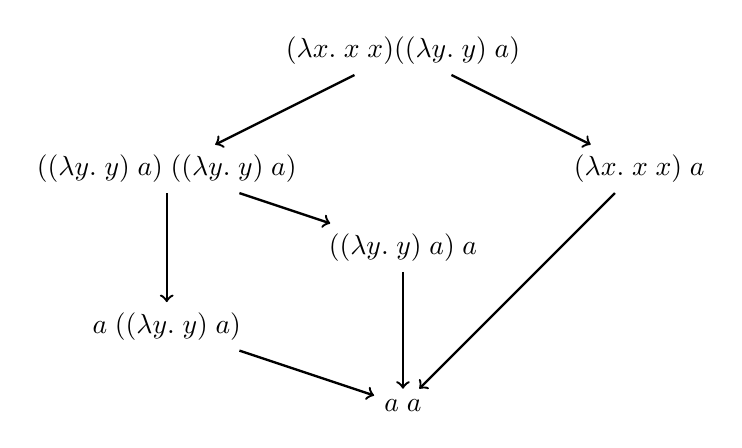
\begin{tikzpicture}[line width=0.3mm]
    \node(T1) at ( 0,  0) {$(\lambda x.\; x\;x)((\lambda y.\;y)\; a)$};
    \node(T2) at (-3, -1.5) {$((\lambda y.\;y)\; a)\;((\lambda y.\;y)\; a)$};
    \node(T3) at ( 3, -1.5) {$(\lambda x.\; x\;x)\;a$};
    \node(T4) at ( 0, -2.5) {$((\lambda y.\;y)\; a)\;a$};
    \node(T5) at (-3, -3.5) {$a\;((\lambda y.\;y)\;a)$};
    \node(T6) at ( 0, -4.5) {$a\;a$};

    \draw[->] (T1) edge (T2) (T2) edge (T4) (T4) edge (T6) (T3) edge (T6)
              (T2) edge (T5) (T5) edge (T6) (T1) edge (T3);
  \end{tikzpicture}
  \end{center}

  This raises the questions : \begin{itemize}
    \item Are some paths better than others ?
    \item Is there always a result in the ? Is it unique ?
  \end{itemize}

  \subsection{Normalization}

  A \textit{normal form} is a term that cannot be reduced anymore,
  formally : $N(t) = \neg \exists t', t \to t' $.

  \exam.

  \begin{tabular}{c|c}
    normal form & not normal form \\
    \hline
    $x$ & $(\lambda x.x)\; y$ \\
    $\lambda x.xy$ & $x\; ((\lambda y.y)\;(\lambda z.zx))$ \\
    $x (\lambda y.y)\;(\lambda z.zx)$ &
  \end{tabular}

  \vspace{0.5cm}

  If $t\to^* t'$ and $t'$ is normal, the term $t'$ is said to be a normal form
  of $t$. This defines our informal notion of a result of a term.

  Some terms do not have a normal form :

  \begin{align*}
    \Omega &= \delta\;\delta \\
          &= (\lambda x.xx)\; (\lambda x.xx) \\
          &\to (xx)\{\lambda x.xx\} \\
          &= x\{\lambda x.xx\}\;x\{\lambda x.xx\} \\
          &= (\lambda x.xx)\; (\lambda x.xx) \\
          &= \Omega
  \end{align*}

  \paragraph{Normalization properties} A term $t$ is :

  \begin{itemize}
    \item \textit{strongly normalizing} if every reduction sequence starting
      from $t$ eventually reaches a normal form :

      \[(\lambda xy.y)\;((\lambda z.z)\;(\lambda z.z))\]

    \item \textit{weakly normalizing}, or normalizable, if there is at least one
      reduction sequence starting from $t$ and reaching a normal form :

      \[(\lambda xy.y)\;((\lambda z.zz)\;(\lambda z.zz))\]
  \end{itemize}

  \subsection{Reduction strategies}

  The purpose of a reduction strategy is to determine a redex reduction order
  within a term. We have two well-known reduction orders :

  \begin{itemize}
    \item \textit{Normal order} : reduce the most external redex first. Apply
      functions without reducing the arguments
    \item \textit{Applicative order} : reduce the most internal redex first.
      Normalize the arguments before reducing the function application itself.
  \end{itemize}

  \exo normal order vs. applicative order.

  Compare normal order reduction and applicative order reduction of the
  following terms :

  \begin{enumerate}
    \item $(\lambda xy.x)\;z\;\Omega$
    \item $(\lambda x.xx)((\lambda y.y)\;z)$
    \item $(\lambda x.x(\lambda y.y)) (\lambda z.(\lambda a.aa)(z\;b))$
  \end{enumerate}

  In each case: does another order allow shorter sequences ?

  \textit{Answer}

  \begin{enumerate}
    \item Normal order
      \begin{align*}
        &(\lambda xy.x)\;z\;\Omega\\
        &\to (\lambda y.z)\; \Omega\\
        &\to z
      \end{align*}

      Applicative order
      \begin{align*}
        &(\lambda xy.x)\;z\;\Omega\\
        &\to (\lambda xy.x)\; \Omega\\
        &\to \ldots
      \end{align*}

      Normal order reduction is as short as possible.

    \item Normal order
      \begin{align*}
        &(\lambda x.xx)\;((\lambda y.y)\;z) \\
        &\to ((\lambda y.y)\; z)\;((\lambda y.y)\;z) \\
        &\to z ((\lambda y.y)\;z) \\
        &\to zz
      \end{align*}

      Applicative order

      \begin{align*}
        &(\lambda x.xx)\;((\lambda y.y)\;z) \\
        &\to (\lambda x.xx)\;z \\
        &\to zz
      \end{align*}

      Applicative order reduction is as short as possible.

    \item Reduction graph :
      \begin{center}
      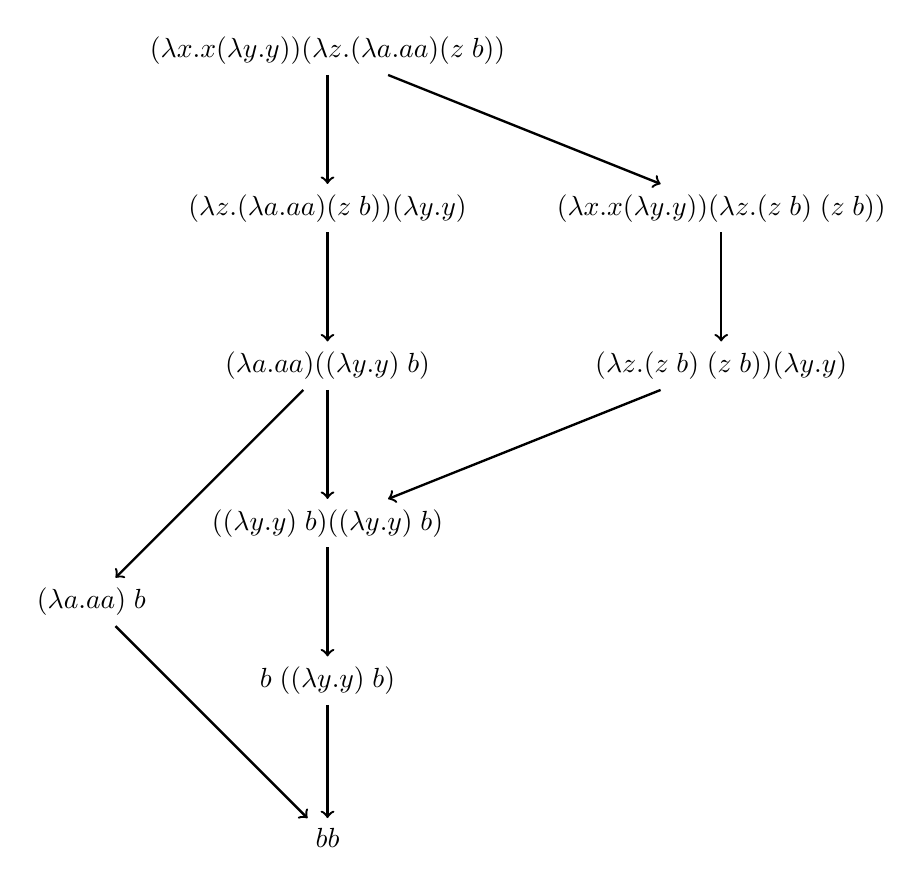
\begin{tikzpicture}[line width=0.3mm]
        \node(T1) at (0, 0) {$(\lambda x.x(\lambda y.y)) (\lambda z.(\lambda a.aa)(z\;b))$};
        \node(T2) at (0, -2) {$(\lambda z.(\lambda a.aa)(z\;b))(\lambda y.y)$};
        \node(T3) at (0, -4) {$(\lambda a.aa)((\lambda y.y)\;b)$};
        \node(T4) at (0, -6) {$((\lambda y.y)\;b)((\lambda y.y)\;b)$};
        \node(T5) at (0, -8) {$b\;((\lambda y.y)\;b)$};
        \node(T6) at (0, -10) {$bb$};

        \node(T7) at (5, -2) {$(\lambda x.x(\lambda y.y)) (\lambda z.(z\;b)\;(z\;b))$};
        \node(T8) at (5, -4) {$(\lambda z.(z\;b)\;(z\;b))(\lambda y.y)$};

        \node(T9) at (-3, -7) {$(\lambda a.aa)\;b$};

        \draw[->] (T1) edge (T2) (T2) edge (T3) (T3) edge (T4) (T4) edge (T5)
                  (T5) edge (T6)
                  (T1) edge (T7) (T7) edge (T8) (T8) edge (T4)
                  (T3) edge (T9) (T9) edge (T6);
      \end{tikzpicture}
      \end{center}

      The middle path is the normal order strategy, the right path is the
      applicative order and the left path is the shortest reduction.
  \end{enumerate}

  \paragraph{Normal order property} If a term $t$ does have a normal form the
  normal order reduction reaches this normal form.

  \subsection{Confluence}

  Confluence is a very useful concept to prove the uniqueness of a result of
  a calculation rule like beta-reduction. It says that if a term can be
  rewritten in more than one way, then there is always a way to revert to a
  common term

  Formally, the confluence is written
  like this: $\forall t\; t_1\; t_2, t \to^* t_1 \wedge t \to^* t_2 \Rightarrow
  \exists u, t_1 \to^* u \wedge t_2 \to^* u$

  We can draw the following diagram:

  \begin{center}
  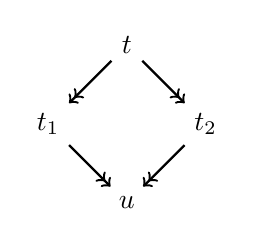
\begin{tikzpicture}[line width=0.3mm]
    \node(t) at (0, 0) {$t$};
    \node(t1) at (-1,-1) {$t_1$};
    \node(t2) at ( 1,-1) {$t_2$};
    \node(u) at ( 0,-2) {$u$};

    \draw[->>](t)  edge (t1)
              (t)  edge (t2)
              (t1) edge (u)
              (t2) edge (u);
  \end{tikzpicture}
  \end{center}

  A rewrite rule can have the \textit{diamond property}. In one rewriting step,
  it can always fall back on the same term in the second rewriting step.
  $\forall t\; t_1\; t_2, t \to t_1 \wedge t_2 \Rightarrow \exists u, t_1 \to u
  \wedge t_2 \to u$

  \begin{center}
  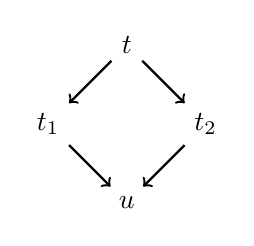
\begin{tikzpicture}[line width=0.3mm]
    \node(t) at (0, 0) {$t$};
    \node(t1) at (-1,-1) {$t_1$};
    \node(t2) at ( 1,-1) {$t_2$};
    \node(u) at ( 0,-2) {$u$};

    \draw[->] (t) edge (t1)
              (t) edge (t2)
              (t1) edge (u)
              (t2) edge (u);
  \end{tikzpicture}
  \end{center}

  \lemma The diamond property implies the confluence.

  \paragraph{proof}
  We can prove that by induction
  on $n + m$ with $n$ the number of steps of $t \to t_1$ and $m$ the number of
  steps of $t \to t_2$.

  \begin{itemize}
    \item $n + m = 0$, then $t = t_1 = t_2$, so $t \not \to t_1$ and $t \not \to
      t_2$ the property is true.

    \item $n + m + 1$ we assume that the diamond property implies the confluence
      on the condition that $t$ reduce to $t_1$ less that $n$ steps and $t$
      reduce to $t_2$ less that $m$ steps.

      \begin{center}
        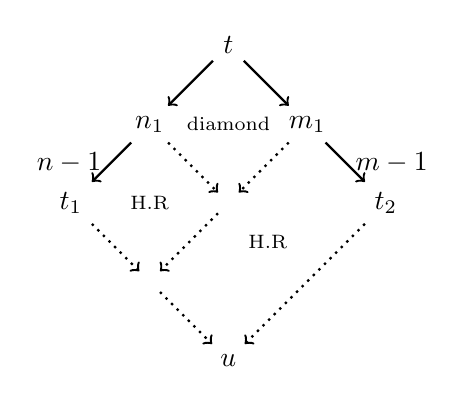
\begin{tikzpicture}[line width=0.3mm]
        \node(t) at (0, 0) {$t$};
        \node(n1) at (-1, -1) {$n_1$};
        \node(m1) at ( 1, -1) {$m_1$};
        \node(t1) at (-2, -2) {$t_1$};
        \node(t2) at ( 2, -2) {$t_2$};
        \node(u)  at ( 0, -4) {$u$};

        \node(nm)  at ( 0, -2) { };
        \node(t1n1)at ( -1, -3) { };

          \draw[->] (t) edge (n1)
                    (t) edge (m1)
                    (n1) edge node[above, left] {$n-1$} (t1)
                    (m1) edge node[above, right] {$m-1$} (t2);

        \draw[->, dotted] (n1) edge (nm) (m1) edge (nm);
        \draw[->, dotted] (t1) edge (t1n1) (nm) edge (t1n1);
        \draw[->, dotted] (t2) edge (u) (t1n1) edge (u);

        \node at (0, -1) {\scriptsize diamond};
        \node at (-1, -2) {\scriptsize H.R};
        \node at (0.5, -2.5) {\scriptsize H.R};

      \end{tikzpicture}
      \end{center}
  \end{itemize}
  \qedsymbol

  The $\beta$-reduction does not have the diamond property :

  \begin{center}
  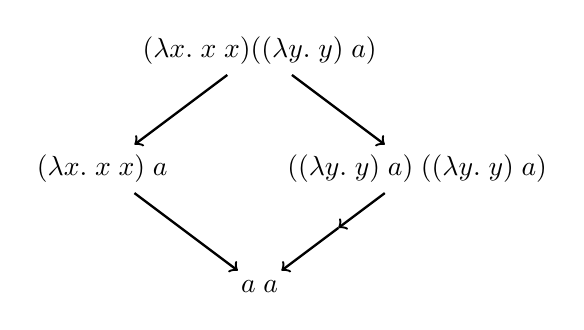
\begin{tikzpicture}[line width=0.3mm]
    \node(T1) at ( 0,  0) {$(\lambda x.\; x\;x)((\lambda y.\;y)\; a)$};
    \node(T3) at (-2, -1.5) {$(\lambda x.\; x\;x)\;a$};
    \node(T2) at ( 2, -1.5) {$((\lambda y.\;y)\; a)\;((\lambda y.\;y)\; a)$};
    \node(T6) at ( 0, -3) {$a\;a$};

    \draw[->] (T1) edge (T3) (T1) edge (T2) (T3) edge (T6)
      (T2) edge ( 1, -2.25)
      (1, -2.25) to (T6);
  \end{tikzpicture}
  \end{center}

  We can proof that the $\beta$-reduction is locally confluent, which is:
  $\forall t\; t_1\; t_2, t \to t_1 \wedge t \to t_2 \Rightarrow \exists u, t_1
  \to ^* u \wedge t_2 \to^* u$. It represents with this diagram :

  \begin{center}
  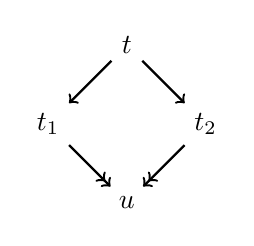
\begin{tikzpicture}[line width=0.3mm]
    \node(t) at (0, 0) {$t$};
    \node(t1) at (-1,-1) {$t_1$};
    \node(t2) at ( 1,-1) {$t_2$};
    \node(u) at ( 0,-2) {$u$};

    \draw[->] (t) edge (t1)
              (t) edge (t2);
    \draw[->>] (t1) edge (u)
               (t2) edge (u);
  \end{tikzpicture}
  \end{center}

  But the local confluence does not imply the confluence, the Curry's counter
  example. This diagram is locally confluent, but it is not confluent.

  \begin{center}
  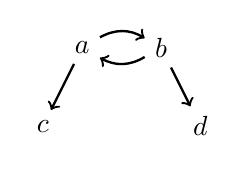
\begin{tikzpicture}[line width=0.3mm]
    \node(a) at (-0.5, 0) {$a$};
    \node(b) at (0.5,0) {$b$};

    \node(c) at (-1,-1) {$c$};
    \node(d) at ( 1,-1) {$d$};

    \draw[->] (a) edge[bend left] (b)
              (b) edge[bend left] (a)
              (a) edge (c)
              (b) edge (d);

  \end{tikzpicture}
  \end{center}

  The proof of confluence is therefore much more complicated than expected.
  We will present two possible proofs.

  \subsubsection{Parallel reduction}

  Parallel reduction proof consists of defining a relation
  $\rightrightarrows_\beta$ that is ``between'' $\to_\beta$ and $\to_\beta^*$.
  This relation need to have the diamond property. Because thanks to this we can
  prove the confluence of this new relation.

  We're going to start by defining the parallel reduction :

  \begin{mathpar}
    \inferrule*[Right=Id]{ }
              { x \\ \rightrightarrows_\beta \\ x} \\

    \inferrule*[Right=Abs]{t \\ \rightrightarrows_\beta \\ t'}
              {\lambda x.t \\ \rightrightarrows_\beta \\ \lambda x.t} \and
    \inferrule*[Right=App]{t_1 \rightrightarrows_\beta t_1' \\ t_2
      \rightrightarrows_\beta t_2' }
              {t_1\;t_2 \\ \rightrightarrows_\beta \\ t_1'\; t_2'} \\
    \inferrule*[Right=Red]{t \rightrightarrows_\beta t' \\ u
    \rightrightarrows_\beta u'}
        {(\lambda x. t) u \rightrightarrows_\beta t'\{x \leftarrow u'\}}
  \end{mathpar}

  \exam $(\lambda x.((\lambda y.y)\;(\lambda z.z))\;x)\;((\lambda w.w)\;a)$

  \begin{mathpar}
    \inferrule*{
      \inferrule*{
        \inferrule*{\inferrule*{ }{y \rightrightarrows_\beta y} \\
          \inferrule*{\inferrule*{ }{z \rightrightarrows_\beta z}}
            {\lambda z.z\rightrightarrows_\beta \lambda z.z}}
          {(\lambda y.y)\;(\lambda z.z)\rightrightarrows_\beta\lambda z.z}
        \\ \inferrule* { }{x\rightrightarrows_\beta x}}
      {(\lambda x.((\lambda y.y)\;(\lambda z.z))\;x)\rightrightarrows_\beta (\lambda z.z)\;x}
    \\
    \inferrule*{\inferrule*{ }{w \rightrightarrows_\beta w} \\
      \inferrule*{ }{a \rightrightarrows_\beta a}}
      {(\lambda w.w)a\rightrightarrows_\beta a}}
     {(\lambda x.((\lambda y.y)\;(\lambda z.z))\;x)\;((\lambda w.w)\;a) \rightrightarrows_\beta (\lambda z.z)\;a}
  \end{mathpar}

  \lemma \label{pid} $\forall t, t \rightrightarrows_\beta t$

  \textit{Proof}: We prove by induction on $t$:

  \begin{itemize}
    \item $t = x$ by definition of $\rightrightarrows_\beta$ we have $x
      \rightrightarrows_\beta a$.
    \item $t = t_1\; t_2$. We have this induction hypothesis $t_1
      \rightrightarrows_\beta t_1$ and $t_2 \rightrightarrows_\beta t_2$. So we
      have $t_1\; t_2 \rightrightarrows_\beta t_1\; t_2$
    \item $t = \lambda x.t_0$. We have this induction hypothesis $t_0
      \rightrightarrows_\beta t_0$. So we have $\lambda x.t_0
      \rightrightarrows_\beta \lambda x.t_0$.
  \end{itemize}
  \qedsymbol

  \lemma $\forall t t', t \to_\beta t' \Rightarrow t \rightrightarrows_\beta
  t'$\hspace{1cm} $\;\to_\beta \subseteq \rightrightarrows_\beta$

  \textit{Proof}: We prove by induction on $\to_\beta$

  \begin{itemize}
    \item Case $(\lambda x.t)\; u \to_\beta t \{x \leftarrow u\}$:

      \begin{mathpar}
        \inferrule*{
          \inferrule*[Left=Lemma-\ref{pid}]{ }{t \rightrightarrows_\beta t} \\
          \inferrule*[Right=Lemma-\ref{pid}]{ }{u \rightrightarrows_\beta u}
        }
          {(\lambda x.t)\; u \rightrightarrows_\beta t \{x \leftarrow u\}}
      \end{mathpar}
    \item Case $t_1\;t_2 \to_\beta t_1'\;t_2$ with $t_1 \to_\beta t_2$. With
      the induction hypothesis $t_1 \rightrightarrows_\beta t_1'$

      \begin{mathpar}
        \inferrule*{\inferrule*[Left=H.R]{ }{t_1\rightrightarrows_\beta t_1'}\\
          \inferrule*[Right=Lemma-\ref{pid}]{ }{t_2 \rightrightarrows_\beta t_2}}
          {t_1\;t_2 \rightrightarrows_\beta t_1'\;t_2}
      \end{mathpar}
    \item The other case are similar.
  \end{itemize}

  \lemma $\forall t t', t \rightrightarrows_\beta t' \Rightarrow t \to_\beta^*
  t'$ \hspace{1cm} $\rightrightarrows_\beta \subseteq \to_\beta^*$

  \textit{Proof}: by induction on $\rightrightarrows_\beta$

  \begin{itemize}
    \item Case $x \rightrightarrows_\beta x$. We have $x\to^0_\beta x$

    \item Case $\lambda x. u \rightrightarrows_\beta \lambda x. u'$ with $t
      \rightrightarrows_\beta t'$. We assume that $t \to_\beta^* t'$ (induction
      hypothesis). We can easily prove by recurrence on the length of
      $\to_\beta^*$, that we have well $\lambda x. t \to_\beta^* \lambda x.t'$

    \item The application rule is similar.

    \item Case $(\lambda x. t)\; u \rightrightarrows_\beta t'\{x \leftarrow
      u'\}$ with $t \rightrightarrows_\beta t'$ and $u \rightrightarrows_\beta
      u'$. Then we have $(\lambda x. t) u \to_\beta^* (\lambda x. t') u$ by
      induction hypothesis on $t$, $(\lambda x. t') u' \to_\beta^* (\lambda x.
      t') u'$ by induction hypothesis on $u$. And finally we have $(\lambda x.
      t') u' \to_\beta t'\{x\leftarrow u'\}$
  \end{itemize}
  \qedsymbol

  \paragraph{method of Tait and Martin-Löf} We want to proof that a relation has
  the diamond property

  \lemma If a relation $\to$ has the diamond property then $\to^*$ has the
  diamond property to.

  \textit{Proof} : We suppose that $\to$ has the diamond property [TODO]
  \qedsymbol

  \lemma If two relation  $\to$ and $\rightrightarrows$ are such that $\to
  \subseteq \rightrightarrows \subseteq \to^*$ then $\rightrightarrows^* =
  \to^*$.

  \textit{Proof}: From $\to \subseteq \rightrightarrows \subseteq \to^*$ we
  deduce $\to^* \subseteq \rightrightarrows^* \subseteq \to^{**}$. However we
  have $\to^* = \to^{**}$. Then $\to^* \subseteq \rightrightarrows
  \subseteq \to^*$ so we have $\rightrightarrows^* = \to^*$.\\
  \qedsymbol

  To proof that $\to^*$ has the diamond property we just need to show that
  $\rightrightarrows_\beta$ has the diamond property. To do this we need the
  following lemma :

  \lemma  \label{dia_iter}
  $a \rightrightarrows_\beta a' \wedge b \rightrightarrows_\beta b'
  \Rightarrow a\{x \leftarrow b\} \rightrightarrows_\beta a'\{x \leftarrow b\}$

  \textit{Proof}:
  By induction one the derivation $a \rightrightarrows_\beta a'$.

  \begin{itemize}
    \item Case $y \rightrightarrows_\beta y$
      \begin{itemize}
        \item If $x = y$, then $x\{x \leftarrow b\} = b \rightrightarrows_\beta
          b' = x\{x \leftarrow b'\}$

        \item If $x \not = y$, then $y\{x \leftarrow b\} = y
          \rightrightarrows_\beta y = y\{x \leftarrow b'\}$
      \end{itemize}

    \item Case $\lambda y. a_0 \rightrightarrows_\beta \lambda y.a_0'$ with $a_0
      \rightrightarrows_\beta a_0'$

      Then $(\lambda y.a_0)\{x\leftarrow b\} = \lambda y. a_0 \{x \leftarrow
      b\}$. By induction hypothesis we have $a_0\{x \leftarrow b\}
      \rightrightarrows_\beta a_0'\{x \leftarrow b'\}$.

      Therefore, we have $\lambda y.a_0\{x\leftarrow b\} \rightrightarrows_\beta
      \lambda y.a_0'\{x\leftarrow b'\} = (\lambda y.a_0')\{x\leftarrow b'\}$

    \item Case $a_1\; a_2 \rightrightarrows_\beta a_1'\;a_2'$ with $a_1
      \rightrightarrows_\beta a_1'$ and $a_2 \rightrightarrows_\beta a_2'$.

      It is similar to the case above.

    \item Case $(\lambda x. a_1)\;a_2\rightrightarrows_\beta (\lambda x.a_1')
      a_2'$ with $a_1 \rightrightarrows_\beta a_1'$ and $a_2
      \rightrightarrows_\beta a_2'$.

      Then $((\lambda y. a_1)a_2)\{x \leftarrow b\} = (\lambda y. a_1\{x
      \leftarrow b\})a_2\{x \leftarrow b\}$.

      By the induction hypothesis we have $a_1\{x \leftarrow b\}
      \rightrightarrows_\beta a_1'\{x \leftarrow b'\}$ and $a_2\{x \leftarrow
      b\} \rightrightarrows_\beta a_2'\{x \leftarrow b'\}$.

      Therefore $(\lambda y. a_1\{x\leftarrow b\})(a_2\{\leftarrow b\})
      \rightrightarrows_\beta (a_1'\{x \leftarrow b'\}\{y \leftarrow a_2'\{x
      \leftarrow b'\}\}$. Thanks to the substitution lemma-\ref{exo:commsubst}

  \end{itemize}
  \qedsymbol

  \lemma $\rightrightarrows_\beta$ has the diamond property.
    $\forall t\; s\; r, t \rightrightarrows_\beta s \wedge t \rightrightarrows_\beta
    r \Rightarrow \exists u, s \rightrightarrows_\beta u \wedge r
    \rightrightarrows_\beta u$.

  \textit{Proof}: By induction on the derivation of $t\rightrightarrows_\beta
  re$.

  \begin{itemize}
    \item Case $x \rightrightarrows_\beta x$. Then $s = x$ so we can take $u =
      x$.

    \item Case $\lambda x.t_0 \rightrightarrows_\beta \lambda x. r_0$ with
      $t_0 \rightrightarrows_\beta r_0$. Then $s = \lambda x. s_0$ with
      $t_0 \rightrightarrows_\beta s_0$.

      By induction hypothesis we have $u_0$ such that $s_0
      \rightrightarrows_\beta u_0$ and $r_0 \rightrightarrows_\beta u_0$.

      Therefore, $\lambda x. s_0 \rightrightarrows_\beta \lambda x. u_0$ And
      $\lambda x. r_0 \rightrightarrows_\beta \lambda x. u_0$

    \item Case $t_1\;t_2 \rightrightarrows_\beta r_1\; r_2$ with $t_1
      \rightrightarrows_\beta r_1$ and $t_2 \rightrightarrows_\beta r_2$.
      Two case for $t_1\;t_2 \rightrightarrows_\beta s_0$:

      \begin{itemize}
        \item if $s = s_1\;s_2$ with $t_1 \rightrightarrows_\beta s_1$ and $t_2
          \rightrightarrows_\beta s_2$ by induction hypothesis there are $u_1$
          and $u_2$ such that $s_1 \rightrightarrows_\beta u_1$, $r_1
          \rightrightarrows_\beta u_1$ and $s_2 \rightrightarrows_\beta u_2$,
          $r_2 \rightrightarrows_\beta u_2$, therefore $s_1s_2
          \rightrightarrows_\beta u_1u_2$ and $r_1r_2
          \rightrightarrows_\beta u_1u_2$.

        \item if $s = s_1\{x \leftarrow s_2\}$ with $t_1 = \lambda x.t_1$ and
          $t_1 \rightrightarrows_\beta s_1$ and $t_2 \rightrightarrows_\beta
          s_2$, then $r_1 = \lambda x.r_1$ with $t_1' \rightrightarrows_\beta
          r_1'$ and by induction hypothesis there are $u_1$ and $u_2$ such that
          $s_1 \rightrightarrows_\beta u_1$ and $r_1'\rightrightarrows_\beta
          u_1$ and $s_2 \rightrightarrows_\beta u_2$ and $r_2
          \rightrightarrows_\beta u_2$.

          Therefore, $(\lambda x.r_1')r_2 \rightrightarrows_\beta u_1\{
            x \leftarrow s_2\}$. And we conclude by the lemma-\ref{dia_iter}
      \end{itemize}

    \item The last case is almost the same.
  \end{itemize}
  \qedsymbol

  \subsubsection{Strip lemma}

  Since confluence is difficult to show due to the infinity of the two branches,
  we define a new property called `strip lemma`. The concept is simple, instead
  of having the relation $\to^*$ on both sides of the confluence we use the
  relation $\to$ and $\to^*$. It is formally defined as follows : $\forall
  t\;t_1\;t_2, t \to t_1 \wedge t \to t_2 \Rightarrow \exists u, t_1 \to^* u
  \wedge t_2 \to^* u$. We can draw this diagram :

  \begin{center}
  \begin{tikzpicture}[line width=0.3mm]
    \node(t) at (0, 0) {$t$};
    \node(t1) at (-1, -1) {$t_1$};
    \node(t2) at ( 2, -1.5) {$t_2$};
    \node(u) at  ( 1,  -2.5) {$u$};

    \draw[->] (t) edge (t1);
    \draw[->>](t) edge (t2);
    \draw[dotted, ->>](t1) edge (u)
                      (t2) edge (u);
  \end{tikzpicture}
  \end{center}

  This property given the confluence :

  \textit{Proof} : We can proof by induction on the length on the left reduction
  (confluence diagram).

  \begin{itemize}
    \item When $n = 0$ is trivial, $t_1 = t$ then $t_1 \to^* t_2$.
    \item For $n + 1$, we have $t \to_{n} t_1' \to t_1$, such that exists $u'$
      with $t_2 \to^* u'$ and $t_1' \to u$ (induction hypothesis).

      We just need to apply the strip lemma to have $u$ such that $t_1 \to u$
      and $u' \to^* u$
  \end{itemize}

  It's easier to understand the proof with this drawing :

  \begin{center}
  \begin{tikzpicture}[line width=0.3mm]
    \node(t) at (0, 0) {$t$};
    \node(t1) at (-1, -1) { };
    \node(t11) at (-2, -2) { };
    \node(t111') at (-3, -3) {$t_1'$};
    \node(t111) at (-4, -4) {$t_1$};

    \node(t2) at  (4, -4) {$t_2$};
    \node(t22) at (3, -5) { };
    \node(t222) at (2, -6) { };
    \node(u') at (1, -7) {$u'$};
    \node(u) at (0, -8) {$u$};

    \draw[->] (t) edge (t1)
              (t1) edge (t11)
              (t111') edge (t111);
    \draw[->>](t) edge (t2);

    \draw[dotted] (t11) edge (t111') (t222) edge (u');
    \draw[dotted, ->>]
          (t1)    edge (t22)
          (t11)   edge (t222)
          (t22)   edge (t222)
          (t111') edge (u')
          (t111)  edge (u)
          (u')    edge (u)
          (t2)    edge (t22);
  \end{tikzpicture}
  \end{center}
  \qedsymbol

  \newpage
  To proof that the $\lambda$-calculus respect the ``strip lemma'' we need to
  define the $\underline{\lambda}$-calculus ($\underline{\Lambda}$ the set of
  $\underline{\lambda}$-terms).

  \defi $\Mlambda$ Set:

  \begin{itemize}
    \item $\forall x \in \text{Var}, x \in \underline{\Lambda}$
    \item $\forall x \in \text{Var}, t \in \underline{\Lambda}, (\lambda x. t) \in \underline{\Lambda}$
    \item $\forall t_1\;t_2 \in \underline{\Lambda}, t_1\;t_2
      \in \underline{\Lambda}$
    \item $\forall x \in \text{Var}, t_1\;t_2 \in \underline{\Lambda},
      (\underline{\lambda} x. t_1)\; t_2 \in \underline{\Lambda}$
  \end{itemize}

  We write $|T|$ the operation who remove every mark on a $\underline
  \lambda$-term.

  \[
    \begin{cases}
      |x| &= x \\
      |\lambda x. t| &= \lambda x. |t| \\
      |t_1\;t_2|     &= |t_1|\; |t_2| \text{\hspace{2cm}if } t_1 \not = \underline \lambda x. t'\\
      |(\underline \lambda x. t_1) \; t_2| &= (\lambda x. |t_1|)\; |t_2|
    \end{cases}
  \]

  We need to define a new substitution and a new rewrite rule :

  \defi Substitution on $\underline \Lambda$

  Substitution is defined as for normal lambda terms. We only add the
  following rule:

  $$((\underline{\lambda}x.t)u)\{y \leftarrow v\} \equiv
  (\underline{\lambda}x.t\{y \leftarrow v\})u\{y \leftarrow v\} $$

  \defi For the $\underline \beta$-reduction we define 2 rules that propagate
  recursively on the other cases :

  $$\beta_0: (\underline \lambda x. t) u \to t\{x \leftarrow u\}$$
  $$\beta_0: (\lambda x. t) u \to t\{x \leftarrow u\}$$


  \defi We define the function $\varphi$ who contract all marked redex on a
  $\mlambda$-term :

  \[
    \begin{cases}
      \varphi(x) &= x \\
      \varphi(u\;v) &= \varphi(u)\;\varphi(v)\text{\hspace{1cm}if }u\not=\mlambda x.t\\
      \varphi(\lambda x. t) &= \lambda x. \varphi(t) \\
      \varphi((\mlambda x. t)\;u) &= \varphi(t)\{x \leftarrow \varphi(u)\}
    \end{cases}
  \]

  \lemma $|t|$ property:
    \label{lemm:abs}

  \begin{enumerate}
    \item $\forall m' \in \mlambda, m n \in \lambda, m' \xrightarrow{|\;|} m
      \wedge M \xrightarrow{\beta} N \Rightarrow \exists N' \in \Mlambda, M'
      \xrightarrow{\mbeta} N' \wedge N' \xrightarrow{|\;|} N$

      \begin{center}
      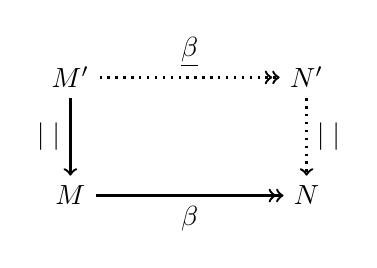
\begin{tikzpicture}[line width=0.3mm]
        \node(M') at (0,  0) {$M'$};
        \node(N') at (3,  0) {$N'$};
        \node(M)  at (0, -1.5) {$M$};
        \node(N)  at (3, -1.5) {$N$};

        \draw[->>, dotted] (M') edge node[above] {$\mbeta$} (N');
        \draw[->,  dotted] (N') edge node[right] {$|\;|$}   (N);
        \draw[->] (M') edge node[left] {$|\;|$}   (M);
        \draw[->>](M)  edge node[below] {$\beta$} (N);
      \end{tikzpicture}
      \end{center}

    \item $\forall m' \in \mlambda, m n \in \lambda, m' \xrightarrow{|\;|} m
      \wedge M \xrightarrow{\beta} N \Rightarrow \exists N' \in \Mlambda, M'
      \xrightarrow{\mbeta} N' \wedge N' \xrightarrow{|\;|} N$

      \begin{center}
      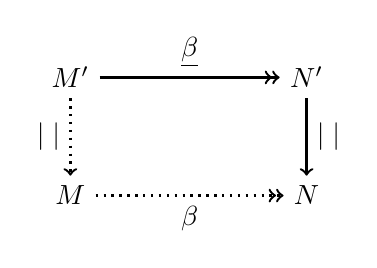
\begin{tikzpicture}[line width=0.3mm]
        \node(M') at (0,  0) {$M'$};
        \node(N') at (3,  0) {$N'$};
        \node(M)  at (0, -1.5) {$M$};
        \node(N)  at (3, -1.5) {$N$};

        \draw[->>] (M') edge node[above] {$\mbeta$} (N');
        \draw[-> ] (N') edge node[right] {$|\;|$}   (N);
        \draw[->,  dotted] (M') edge node[left]  {$|\;|$} (M);
        \draw[->>, dotted] (M)  edge node[below] {$\beta$} (N);
      \end{tikzpicture}
      \end{center}
  \end{enumerate}
  \textit{Proof}:
    \begin{enumerate}
      \item We proceed by induction on the reduction $M \rsbeta N$.
        \begin{itemize}
          \item $M \rsbeta M$, then $M = N$. We just take $M' = M$ (easy).
          \item $M \rbeta M_t$ and $M_t \rsbeta N$. By induction hypothesis we
            have $M_t'$ such that $|M_t'| = M_t $ and $M_t' \rsbeta N'$.

            The reduction $M' \to_\mbeta M'_t$ exists, we can contract the same
            redex (if it was marked we would contract the new unmarked).

            So we have $M' \to_\mbeta M'_t \to_\mbeta N' \xrightarrow{|\;|} N$
        \end{itemize}
      \item Similar.
    \end{enumerate}
  \qedsymbol

  \lemma $\varphi$ property
    \label{lemm:phi}

    \begin{enumerate}
      \item $\forall u v \in \Mlambda, \varphi(u\{x \leftarrow v\}) =
        \varphi(u)\{x \leftarrow \varphi(v)\}$

      \item $\forall M N \in \Mlambda, M \tosmbeta N \Rightarrow \varphi(M)
        \rsbeta \varphi(N)$

        \begin{center}
        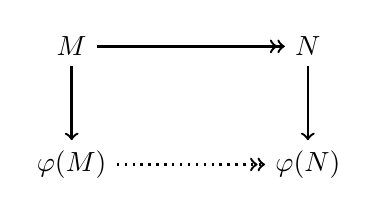
\begin{tikzpicture}[line width=0.3mm]
          \node(M)  at (0, 0) {$M$};
          \node(N)  at (3, 0) {$N$};
          \node(PM) at (0, -1.5) {$\varphi(M)$};
          \node(PN) at (3, -1.5) {$\varphi(N)$};

          \draw[->] (M) edge (PM) (N) edge (PN);
          \draw[->>] (M) edge (N);
          \draw[->>, dotted] (PM) edge (PN);
        \end{tikzpicture}
        \end{center}
    \end{enumerate}
    \textit{Proof}:
      \begin{enumerate}
        \item We proceed by induction on the term $u$.

          \begin{itemize}
            \item Case $u = z$
              \begin{itemize}
                \item if $z = x$, then
                  $\varphi(x\{x \leftarrow v\}) = \varphi(v) = \varphi(x)\{x
                  \leftarrow \varphi(v)\}$
                \item if $z \not = x$, then
                  $\varphi(z\{x \leftarrow v\}) = z = \varphi(z)\{x
                  \leftarrow \varphi(v)\}$
              \end{itemize}

            \item Case $t = \lambda y. t_0$,
              \begin{align*}
                \varphi((\lambda y. t_0)\{x \leftarrow v\})
                &= \varphi(\lambda y. t_0\{x \leftarrow v\}) \\
                &= \lambda y. \varphi(t_0\{x \leftarrow v\}) & \text{By
                convention} \\
                &= \lambda y. \varphi(t_0)\{x\leftarrow \varphi(v)\} & \text{By
                induction hypothesis} \\
                &= \varphi(\lambda y.t_0)\{x\leftarrow \varphi(v)\}
              \end{align*}

            \item Case $t = t_1\;t_2$
              \begin{align*}
                \varphi((t_1\;t_2)\{x \leftarrow v\})
                &= \varphi(t_1\{x \leftarrow v\}) (\varphi(t_2\{x \leftarrow v\})) \\
                &= \varphi(t_1)\{x \leftarrow \varphi(v)\} \varphi(t_2)\{x
                  \leftarrow \varphi(v)\}) & \text{By induction hypothesis}\\
                &= (\varphi(t_1)\;\varphi(t_2)) \{x \leftarrow \varphi(v)\}) \\
                &= (\varphi(t_1\;t_2)) \{x \leftarrow \varphi(v)\}) \\
              \end{align*}

            \item Case $t=(\mlambda y. t_0)\;t_1$
              \begin{align*}
                \varphi(((\mlambda y. t_0)\;t_1)\{x \leftarrow v\})
                &=\varphi((\mlambda y. t_0\{x \leftarrow v\})\;t_1\{x
                \leftarrow v\}) \\
                &=\varphi(t_0\{x \leftarrow v\})\{y\leftarrow \varphi(t_1\{x
                \leftarrow v\})\} \\
                &=\varphi(t_0)\{x \leftarrow \varphi(v)\})\{y\leftarrow
                \varphi(t_1)\{x \leftarrow \varphi(v)\}\} & \text{By induction
                hypothesis}\\
                &=\varphi(t_0)\{y\leftarrow \varphi(t_1)\}
                            \{x \leftarrow \varphi(v)\} & \text{By the lemma
                            \ref{exo:commsubst}}\\
                &=\varphi((\mlambda y. t_0)\; t_1)\{x \leftarrow \varphi(v)\}
             \end{align*}
          \end{itemize}
        \item By induction on $\tosmbeta$, using $(1)$
      \end{enumerate}
    \qedsymbol

  \newpage
  \lemma \label{lemma:bar-phi}
  $\forall t, |t| \rsbeta \varphi(t)$

  \begin{center}
    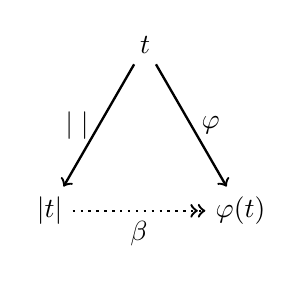
\begin{tikzpicture}[line width=0.3mm, scale=1.4]
    \node(t) at (90:1) {$t$};
    \node(bt) at (210:1) {$|t|$};
    \node(pt) at (330:1) {$\varphi(t)$};

    \draw[->] (t) edge node[left] {$|\;|$} (bt)
              (t) edge node[right] {$\varphi$} (pt);
    \draw[->>, dotted] (bt) edge node[below] {$\beta$} (pt);
  \end{tikzpicture}
  \end{center}
  \textit{Proof}: We will show our property by induction on the term $t$.
  \begin{itemize}
    \item Case $t = x$, $|x| = x = \varphi(x)$, so we have $|t| \to_\beta^0
      \varphi(t)$.
    \item Case $t = \lambda x. t_0$, by the induction hypothesis we know that
      $|t_0| \rsbeta \varphi(t_0)$.
      \begin{align*}
        |(\lambda x. t_0)| &= \lambda x. |t_0| \\
        &\rsbeta \lambda x. \varphi(t_0) & \text{By induction hypothesis} \\
        &= \varphi(\lambda x. t_0)
      \end{align*}

    \item Case $t = t_1\; t_2$, by the induction hypothesis we know that
      $|t_1| \rsbeta \varphi(t_1)$ and $|t_2| \rsbeta \varphi(t_2)$.
      \begin{align*}
        |t_1\;t_2| &= |t_1|\;|t_2| \\
        &\rsbeta \varphi(t_1)\;\varphi(t_2) & \text{By induction hypothesis} \\
        &= \varphi(t_1\;t_2)
      \end{align*}

    \item Case $t=(\mlambda x. t_0)\;t_1$, by the induction hypothesis we know that
      $|t_0| \rsbeta \varphi(t_0)$ and $|t_1| \rsbeta \varphi(t_1)$.

        \begin{align*}
          |(\mlambda x. t_0)\;t_1| &= (\lambda x. |t_0|)\;|t_1| \\
            &\rsbeta (\lambda x. \varphi(t_0))\;\varphi(t_1) & \text{By
            induction hypothesis}\\
            &\to \varphi(t_0)\{x \leftarrow \varphi(t_1)\} \\
            &=\varphi((\mlambda x. t_0)\;t_1)
        \end{align*}

  \end{itemize}

  \qedsymbol

  \newpage
  \lemma Strip-lemma:

   $$\forall t\;t_1\;t_2, t \to t_1 \wedge t \to t_2 \Rightarrow \exists u, t_1
   \to^* u \wedge t_2 \to^* u$$

  \begin{center}
  \begin{tikzpicture}[line width=0.3mm]
    \node(t) at (0, 0) {$t$};
    \node(t1) at (-1, -1) {$t_1$};
    \node(t2) at ( 2, -1.5) {$t_2$};
    \node(u) at  ( 1,  -2.5) {$u$};

    \draw[->] (t) edge (t1);
    \draw[->>](t) edge (t2);
    \draw[dotted, ->>](t1) edge (u)
                      (t2) edge (u);
  \end{tikzpicture}
  \end{center}

  \textit{Proof}:
    Let $t'$, such that $|t'| = t$ and $\varphi(t') = t_1$. By hypothesis, we
    know that, $t \rsbeta t_2$, so we have by the Lemma-\ref{lemm:abs} $t_2' \in
    \Mlambda$ with $|t_2'| = t_2$. We take $u = \varphi(t_2')$.

    Then by the Lemma-\ref{lemm:phi}, we have
    $t_1 \rsbeta u$ and $\varphi(t_2') = u$. We finally have $t_2' \rsbeta u$
    thanks to the Lemma-\ref{lemma:bar-phi}.

    We can resume this proof with the diagram below:

    \begin{center}
    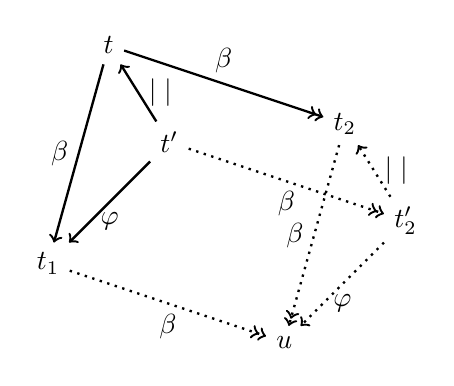
\begin{tikzpicture}[line width=0.3mm]
      \node(t)  at (0, 0, 0) {$t$};
      \node(t') at (0, -2,-2) {$t'$};
      \node(t1) at (0, -2, 2) {$t_1$};

      \node(t2)  at (3, -1, 0) {$t_2$};
      \node(t2') at (3, -3,-2) {$t_2'$};
      \node(u)   at (3, -3, 2) {$u$};

      \draw[->](t') edge node[right] {$|\;|$} (t)
               (t') edge node[below] {$\varphi$} (t1)
               (t)  edge node[left]  {$\beta$} (t1);
      \draw[->>](t) edge node[above] {$\beta$} (t2);
      \draw[->>, dotted] (t') edge node[below] {$\beta$} (t2');
      \draw[->>, dotted](t1) edge node[below] {$\beta$} (u);
      \draw[->>, dotted] (t2) edge node[left]  {$\beta$} (u);
      \draw[->,  dotted](t2')edge node[right] {$|\;|$}    (t2);
      \draw[->,  dotted](t2')edge node[below] {$\varphi$} (u);
    \end{tikzpicture}
    \end{center}

    Resume:
    \begin{enumerate}
      \item Lemma-\ref{lemm:abs}, give $t_2'$ : $t' \rsbeta t_2'$ and $|t_2'| =
        t_2$.
      \item Lemma-\ref{lemma:bar-phi}, give $t_2 \rsbeta \varphi(t_2') = u$.
      \item Lemma-\ref{lemm:phi}, give $t_1 \rsbeta \varphi(t_2') = u$
    \end{enumerate}

  \qedsymbol


  \subsubsection{Church-Rosser theorem}

  If $t_1 =_\beta t_2$ the there is $u$ such that $t_1 \to_\beta^* u$ and $t_2
  \to_\beta^* u$

  Consequences :

  \begin{itemize}
    \item if $t$ has a normal form $n$ then $t \to_\beta^* n$

    \item any $\lambda$-term can has only one normal form

    \item if two normal form $n$ and $m$ are syntactically different, then $n
      \not =_\beta m$.
  \end{itemize}




\end{document}
